\documentclass[11pt,a4paper]{article}

%==============================================================================
% PACKAGES AND PAGE GEOMETRY
%==============================================================================
\usepackage[a4paper,top=2.3cm,bottom=2.3cm,left=2.1cm,right=2.1cm,headheight=14pt]{geometry}
\usepackage[utf8]{inputenc}
\usepackage[T1]{fontenc}
\usepackage{lmodern}
\usepackage{microtype}
\usepackage{amsmath,amssymb,amsfonts}
\usepackage{booktabs}
\usepackage{tabularx}
\usepackage{array}
\usepackage{enumitem}
\usepackage[table]{xcolor}
\usepackage{graphicx}
\usepackage{adjustbox}
\usepackage{pifont}
\usepackage{tikz}
\usetikzlibrary{arrows.meta,positioning,fit,backgrounds,calc,shapes.geometric,decorations.pathreplacing}
\usepackage[most]{tcolorbox}
\usepackage{fancyhdr}
\usepackage[nobottomtitles]{titlesec}
\usepackage{caption}
\usepackage[section]{placeins}
\usepackage[bookmarks=false]{hyperref}

\linespread{1.07}
\setlength{\parskip}{3pt}
\setlength{\parindent}{0pt}
\emergencystretch=2em

%==============================================================================
% COLOUR PALETTE
%==============================================================================
\definecolor{primarynavy}{RGB}{20,35,75}
\definecolor{accentteal}{RGB}{0,128,128}
\definecolor{darkslate}{RGB}{45,55,72}
\definecolor{lightgreybg}{RGB}{245,247,251}
\definecolor{bordergrey}{RGB}{203,213,225}
\definecolor{crimsonred}{RGB}{180,40,40}
\definecolor{forestgreen}{RGB}{34,139,34}
\definecolor{amberorange}{RGB}{217,119,6}

\hypersetup{
  bookmarks=false,
  colorlinks=true, linkcolor=primarynavy, citecolor=accentteal, urlcolor=accentteal,
  pdfauthor={Vedant Panchal (23AIML042), Dax Virani (23AIML076)},
  pdftitle={MIRAGE 3.0: AI Execution Assurance Platform - Project Master Technical Report},
  pdfsubject={Project Review Report - CSPIT, Dept. of AI and ML}
}

%==============================================================================
% HEADINGS, HEADERS, CAPTIONS
%==============================================================================
\titleformat{\section}{\color{primarynavy}\sffamily\Large\bfseries}{\thesection}{0.8em}{}[{\color{primarynavy}\titlerule[0.8pt]}]
\titleformat{\subsection}{\color{accentteal}\sffamily\large\bfseries}{\thesubsection}{0.8em}{}
\titleformat{\subsubsection}{\color{darkslate}\sffamily\normalsize\bfseries}{\thesubsubsection}{0.8em}{}
\titlespacing*{\section}{0pt}{16pt}{8pt}
\titlespacing*{\subsection}{0pt}{12pt}{5pt}

\pagestyle{fancy}
\fancyhf{}
\renewcommand{\headrulewidth}{0.4pt}
\renewcommand{\footrulewidth}{0.4pt}
\fancyhead[L]{\small\sffamily\color{darkslate}\textbf{MIRAGE 3.0} -- AI Execution Assurance Platform}
\fancyhead[R]{\small\sffamily\color{darkslate}CSPIT -- Dept.\ of AI \& ML}
\fancyfoot[L]{\small\sffamily\color{darkslate}V.\ Panchal (23AIML042) \& D.\ Virani (23AIML076)}
\fancyfoot[R]{\small\sffamily\color{darkslate}Page \thepage}

\captionsetup{font=small,labelfont={bf,color=primarynavy},skip=6pt}

%==============================================================================
% TABLE HELPERS
%==============================================================================
\newcolumntype{L}[1]{>{\raggedright\arraybackslash}p{#1}}
\newcolumntype{Y}{>{\raggedright\arraybackslash}X}
\newcommand{\hc}[1]{\textcolor{white}{\textbf{#1}}}
\newcommand{\hdrrow}{\rowcolor{primarynavy}}
\newcommand{\stImpl}{\textcolor{forestgreen}{\textbf{Implemented}}}
\newcommand{\stPart}{\textcolor{amberorange}{\textbf{Partial}}}
\newcommand{\stSpec}{\textcolor{darkslate}{\textbf{Specification}}}
\newcommand{\stFut}{\textcolor{primarynavy}{\textbf{Roadmap}}}
\newcommand{\fp}[1]{\texttt{\scriptsize #1}}
\newcommand{\cmark}{\textcolor{forestgreen}{\ding{51}}}
\newcommand{\xmark}{\textcolor{crimsonred}{\ding{55}}}

%==============================================================================
% CALLOUT BOXES
%==============================================================================
\newtcolorbox{infobox}[2]{enhanced,breakable,colback=#1!4!white,colframe=#1,coltitle=white,
  fonttitle=\sffamily\bfseries\small,title={#2},arc=2mm,boxrule=0.8pt,
  left=3mm,right=3mm,top=2mm,bottom=2mm}

%==============================================================================
% TIKZ STYLE LIBRARY (shared by every figure)
%==============================================================================
\tikzset{
  base/.style={font=\sffamily\scriptsize, align=center, inner sep=3pt, text=darkslate},
  box/.style={base, rectangle, rounded corners=2pt, draw=primarynavy, fill=white, line width=0.6pt, minimum height=8mm, minimum width=2.4cm},
  ctrl/.style={box, fill=primarynavy!8},
  gate/.style={box, draw=crimsonred, fill=crimsonred!8},
  store/.style={box, draw=accentteal, fill=accentteal!10},
  ok/.style={box, draw=forestgreen, fill=forestgreen!12},
  bad/.style={box, draw=crimsonred, fill=crimsonred!10},
  warn/.style={box, draw=amberorange, fill=amberorange!14},
  dec/.style={base, diamond, aspect=2.4, draw=amberorange, fill=amberorange!10, line width=0.6pt, inner sep=1pt},
  note/.style={base, rectangle, draw=bordergrey, fill=lightgreybg, rounded corners=1pt, font=\sffamily\tiny},
  arr/.style={-{Stealth[length=2.2mm,width=1.8mm]}, line width=0.7pt, draw=primarynavy},
  arrd/.style={arr, dashed},
  arrr/.style={arr, draw=crimsonred},
  arr2/.style={line width=0.7pt, draw=primarynavy, arrows={Stealth[length=2.2mm,width=1.8mm]-Stealth[length=2.2mm,width=1.8mm]}},
  lbl/.style={font=\sffamily\tiny, text=darkslate, inner sep=1.5pt, fill=white},
  plane/.style={rectangle, rounded corners=3pt, draw=#1, fill=#1!6, line width=0.8pt, inner sep=7pt},
  planelabel/.style={font=\sffamily\scriptsize\bfseries},
}
\newcommand{\dotp}[2]{\fill[primarynavy] (#1,#2) circle (0.14);}
\newcommand{\dotr}[2]{\draw[primarynavy,line width=0.8pt,fill=white] (#1,#2) circle (0.14);}
\newcommand{\msg}[4]{\draw[arr] (#1,#3) -- node[above,font=\sffamily\tiny,inner sep=1.5pt]{#4} (#2,#3);}
\newcommand{\msgd}[4]{\draw[arrd] (#1,#3) -- node[above,font=\sffamily\tiny,inner sep=1.5pt]{#4} (#2,#3);}

%==============================================================================
\begin{document}
%==============================================================================

\pagenumbering{roman}

%------------------------------------------------------------------------------
% TITLE PAGE
%------------------------------------------------------------------------------
\begin{titlepage}
\thispagestyle{empty}
\centering
\vspace*{0.2cm}
{\Large\scshape Chandubhai S.\ Patel Institute of Technology (CSPIT)\par}
\vspace{0.15cm}
{\large\scshape Department of Artificial Intelligence and Machine Learning\par}
\vspace{0.15cm}
{\normalsize\scshape Charotar University of Science and Technology (CHARUSAT)\par}
\vspace{0.6cm}

{\color{primarynavy}\rule{\linewidth}{1.5pt}}\\[0.4cm]
{\sffamily\huge\bfseries\color{primarynavy} PROJECT MASTER TECHNICAL REPORT\par}
\vspace{0.3cm}
{\sffamily\Large\bfseries\color{accentteal} MIRAGE 3.0: AI Execution Assurance Platform\par}
\vspace{0.2cm}
{\normalsize\color{darkslate}\textbf{A Unified Architecture for Governed AI Transactions, Capability Enforcement, and Epistemic Reality Verification}\par}
\vspace{0.3cm}
{\color{primarynavy}\rule{\linewidth}{1.5pt}}\\[0.5cm]

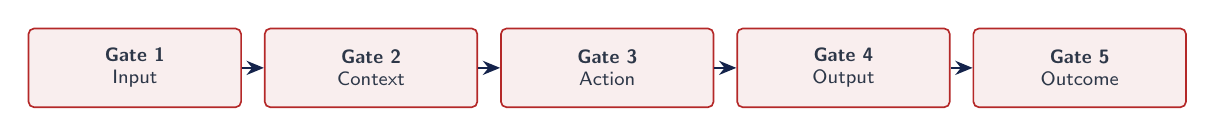
\begin{tikzpicture}
  \foreach \i/\t in {0/Input,1/Context,2/Action,3/Output,4/Outcome}{
    \node[gate,minimum width=2.7cm,minimum height=1.0cm] (tg\i) at (\i*3.0,0) {\textbf{Gate \the\numexpr\i+1\relax}\\\t};
  }
  \foreach \i in {0,1,2,3}{
    \pgfmathtruncatemacro{\j}{\i+1}
    \draw[arr] (tg\i) -- (tg\j);
  }
\end{tikzpicture}

\vspace{0.6cm}
\begin{tcolorbox}[colback=lightgreybg,colframe=primarynavy,arc=2mm,boxrule=0.8pt,width=\linewidth]
\centering\sffamily\textbf{\large Project Metadata and Student Investigators}\\[0.2cm]
\small
\begin{tabularx}{\linewidth}{@{}L{4.0cm}Y@{}}
\textbf{Student Investigator 1:} & Vedant Panchal (ID: 23AIML042)\\[2pt]
\textbf{Student Investigator 2:} & Dax Virani (ID: 23AIML076)\\[2pt]
\textbf{Degree Program:} & Bachelor of Technology in Artificial Intelligence \& Machine Learning\\[2pt]
\textbf{Department / College:} & Dept.\ of AI \& ML, CSPIT, CHARUSAT\\[2pt]
\textbf{Academic Year:} & 2026--2027\\[2pt]
\textbf{Project Category:} & Enterprise AI Safety, Autonomous Execution Assurance, Robust Systems\\[2pt]
\textbf{Engineering Status:} &
  Perimeter security hardened (all three P0 vulnerabilities closed).\newline
  Gates 1 and 4 implemented and validated; transaction scaffolding in progress.\newline
  Live multi-signal verification validated (\texttt{LIVE\_DEMO\_READY}).\newline
  Submitted for faculty review and approval.
\end{tabularx}
\end{tcolorbox}
\vfill
{\small\color{darkslate} Report date: October 2026\par}
\end{titlepage}

%------------------------------------------------------------------------------
% ABSTRACT
%------------------------------------------------------------------------------
\begin{abstract}
\noindent As AI systems evolve from conversational assistants into autonomous agents that call tools, query databases and trigger consequential actions, hallucination detection alone no longer bounds enterprise risk. An agent that can write to a database, issue a payment or exfiltrate private context fails in ways that a text-level check cannot see.

\textbf{MIRAGE 3.0} is an \emph{AI Execution Assurance Platform}: a mediation fabric between AI systems and the external world, built on the promise \emph{``Control AI before it acts. Verify AI after it acts.''} Every agent interaction is wrapped in a governed \textbf{AI Transaction} and evaluated across \textbf{five assurance gates}: (1)~Input Assurance (identity, capabilities, prompt-injection defence, DLP); (2)~Context Assurance (retrieval provenance, memory integrity, information-flow control with taint tracking); (3)~Action Assurance (schema conformance, pre-execution invariants, sliding-window blast-radius limits); (4)~Output Assurance (atomic claim decomposition; fusion of Qdrant retrieval, Groq self-consistency sampling and DeBERTa-v3 NLI; split-conformal calibration at $1-\alpha=0.95$; LangGraph self-healing); and (5)~Outcome Assurance (Epistemic Reality Verification across seven states).

After a pre-implementation security audit that found and closed three critical P0 identity-boundary vulnerabilities, this report presents the architecture, mathematical formulation, live telemetry from Groq/Qdrant/PostgreSQL runs, a competitive comparison, a strictly honest implementation inventory, and a phased roadmap for faculty review.
\end{abstract}

\begin{infobox}{accentteal}{Reading guide: what is built and what is specified}
Throughout this report, components carry one of four labels, summarised in Table~\ref{tab:implementation_inventory} and Figure~\ref{fig:status}:
\stImpl{} (running and tested), \stPart{} (scaffolding exists, integration under way), \stSpec{} (designed and documented, not yet coded), and \stFut{} (scheduled work). Gates~1 and~4 are implemented; Gates~2, 3 and~5 are currently specifications.
\end{infobox}

\vfill
{\small\color{darkslate}\textbf{Keywords:} AI execution assurance, governed AI transactions, epistemic reality verification, assurance gates, split-conformal prediction, information-flow control, LangGraph self-correction, multi-tenant security.}

\clearpage
\tableofcontents
\clearpage
\listoffigures
\clearpage
\listoftables
\clearpage
\pagenumbering{arabic}

%==============================================================================
\section{Executive Summary and Strategic Reset}
%==============================================================================

\subsection{From hallucination detector to assurance fabric}
MIRAGE 2.x was a hallucination detector: it decomposed model completions into claims and scored factual consistency using retrieval, sampling and entailment signals. That scope is scientifically sound but no longer sufficient. Production agents now use tool protocols (Model Context Protocol, function calling), long-term vector memory, code interpreters and internal APIs. In that setting:
\begin{itemize}[leftmargin=*,itemsep=1pt]
  \item a factually accurate reply can still carry out an unauthorised database drop;
  \item a polite completion can be the by-product of an indirect prompt injection that leaked tenant secrets;
  \item an agent can claim an API call succeeded when it timed out, or claim failure when it partly mutated production state.
\end{itemize}

\begin{infobox}{primarynavy}{The MIRAGE 3.0 product statement}
MIRAGE is not merely a hallucination detector, gateway, observability dashboard or guardrail wrapper. It is an \textbf{AI Execution Assurance Platform}.

\medskip
\textit{``MIRAGE sits between AI systems and the real world, inspecting inputs, context, actions, outputs and outcomes to enforce identity, security, policy, reliability and cost controls, while using adaptive verification and model routing to reach the required level of assurance at the lowest practical cost.''}

\medskip
\textbf{Operational promise:} \emph{Control AI before it acts. Verify AI after it acts.}
\end{infobox}

All scientific assets of MIRAGE 2.x are preserved: retrieval-augmented verification (RAV), self-consistency sampling (SCS), natural language inference (NLI), visual grounding (VGS), the Hallucination Risk Score (HRS), isotonic and Mondrian split-conformal calibration \cite{vovk2005,lei2018}, TreeSHAP attribution \cite{lundberg2020}, and LangGraph self-healing. They are repositioned as the \emph{Verification Engine} inside Gate~4 (Figure~\ref{fig:evolution}).

\begin{figure}[!htbp]
\centering
\begin{adjustbox}{max width=\linewidth}
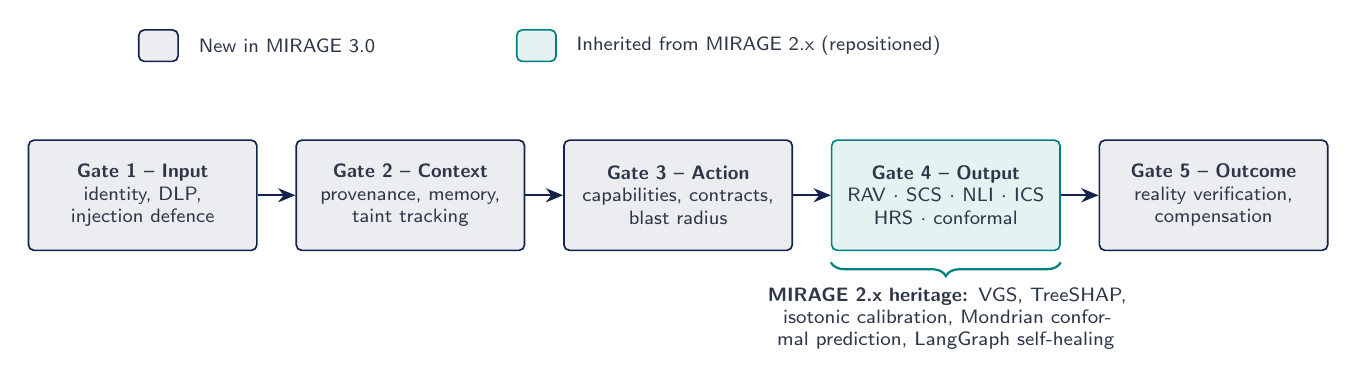
\begin{tikzpicture}
  % legend
  \node[ctrl,minimum width=0.5cm,minimum height=0.4cm] at (0.2,1.9) {};
  \node[base,anchor=west] at (0.6,1.9) {New in MIRAGE 3.0};
  \node[store,minimum width=0.5cm,minimum height=0.4cm] at (5.0,1.9) {};
  \node[base,anchor=west] at (5.4,1.9) {Inherited from MIRAGE 2.x (repositioned)};
  % gates
  \node[ctrl,minimum width=2.9cm,minimum height=1.4cm] (g1) at (0,0)    {\textbf{Gate 1 -- Input}\\identity, DLP,\\injection defence};
  \node[ctrl,minimum width=2.9cm,minimum height=1.4cm] (g2) at (3.4,0)  {\textbf{Gate 2 -- Context}\\provenance, memory,\\taint tracking};
  \node[ctrl,minimum width=2.9cm,minimum height=1.4cm] (g3) at (6.8,0)  {\textbf{Gate 3 -- Action}\\capabilities, contracts,\\blast radius};
  \node[store,minimum width=2.9cm,minimum height=1.4cm] (g4) at (10.2,0) {\textbf{Gate 4 -- Output}\\RAV $\cdot$ SCS $\cdot$ NLI $\cdot$ ICS\\HRS $\cdot$ conformal};
  \node[ctrl,minimum width=2.9cm,minimum height=1.4cm] (g5) at (13.6,0) {\textbf{Gate 5 -- Outcome}\\reality verification,\\compensation};
  \foreach \a/\b in {g1/g2,g2/g3,g3/g4,g4/g5}{\draw[arr] (\a) -- (\b);}
  \draw[decorate,decoration={brace,mirror,amplitude=5pt},accentteal,line width=0.8pt]
    ([yshift=-4pt]g4.south west) -- ([yshift=-4pt]g4.south east);
  \node[base,text width=6cm,below=10pt of g4] {\textbf{MIRAGE 2.x heritage:} VGS, TreeSHAP, isotonic calibration, Mondrian conformal prediction, LangGraph self-healing};
\end{tikzpicture}
\end{adjustbox}
\caption{Scope expansion from MIRAGE 2.x (Gate~4 only) to MIRAGE 3.0 (five gates).}
\label{fig:evolution}
\end{figure}

%==============================================================================
\section{Problem Statement: Fourteen AI Execution Failure Modes}
%==============================================================================

\subsection{From chat verification to action assurance}
Between 2022 and 2024 the central enterprise question was \emph{``Was the answer factually correct?''} For autonomous agents the question becomes: \emph{Was the agent permitted to take that action, did it stay inside its capability boundary, did the action really happen, and is production left in a consistent state?}

Conventional guardrails (regex matchers, prompt wrappers, LLM-as-judge classifiers) treat interactions as isolated strings. They lack a transaction concept, cannot enforce identity boundaries, cannot track provenance across multi-turn reasoning, and cannot confirm that external side effects occurred.

\subsection{Taxonomy of failure modes}
\begin{table}[!htbp]
\centering\small
\renewcommand{\arraystretch}{1.2}
\rowcolors{2}{white}{lightgreybg}
\begin{tabularx}{\linewidth}{@{}r L{3.2cm} L{4.5cm} Y@{}}
\hdrrow \hc{\#} & \hc{Failure mode} & \hc{Mechanism} & \hc{MIRAGE 3.0 countermeasure}\\
\toprule
1 & Unauthenticated agent identity & Agents call tools with forged or ambient credentials. & Cryptographic JWT/API identity resolution; ASGI header stripping.\\
2 & Direct or indirect prompt injection & Adversarial instructions in queries or external documents override system goals. & Gate~1 deterministic preflight and semantic jailbreak filters.\\
3 & Sensitive data exfiltration (DLP) & PII, credentials or IP leak via completions or tool calls. & Information-flow control with taint tracking; egress policy.\\
4 & Context and retrieval poisoning & Adversarial or stale RAG chunks corrupt reasoning. & Gate~2 provenance, freshness and integrity checks.\\
5 & Excessive agency & Agent attempts operations beyond its charter. & Capability-based security with default-deny governance.\\
6 & Malformed tool parameters & Invalid types, SQL injection, unconstrained file paths. & Gate~3 schema validation and pre-execution invariants.\\
7 & Blast-radius accumulation & Low-risk micro-actions add up to catastrophic damage. & Sliding-window cumulative risk accounting.\\
8 & Extrinsic factual fabrication & Generation invents facts unsupported by references. & Gate~4 RAV over Qdrant.\\
9 & Stochastic semantic dispersion & Epistemic uncertainty yields diverging samples. & Parallel Groq self-consistency sampling.\\
10 & Logical contradiction & Claims contradict authoritative ground truth. & DeBERTa-v3 cross-encoder NLI.\\
11 & Visual / multimodal discrepancy & Text describes objects absent from the image. & OpenCLIP similarity and LLaVA-1.6 consistency.\\
12 & Epistemic reality discrepancy & Agent asserts success but the world is unchanged. & Gate~5 postcondition probes against ground truth.\\
13 & Partial failure without compensation & Multi-step workflow fails midway leaving side effects. & Transaction lifecycle with compensation and rollback.\\
14 & Non-repudiation and audit failure & Cannot prove who authorised what, or on what evidence. & Tamper-evident SHA-256 hash-chained audit ledger.\\
\bottomrule
\end{tabularx}
\caption{The fourteen failure modes addressed by MIRAGE 3.0.}
\label{tab:14_failures}
\end{table}

Figure~\ref{fig:traceability} traces each failure mode to the gate(s) that own it. Every failure mode has at least one primary owner, and failure mode~14 is cross-cutting through the audit ledger.

\begin{figure}[!htbp]
\centering
\begin{adjustbox}{max width=\linewidth}
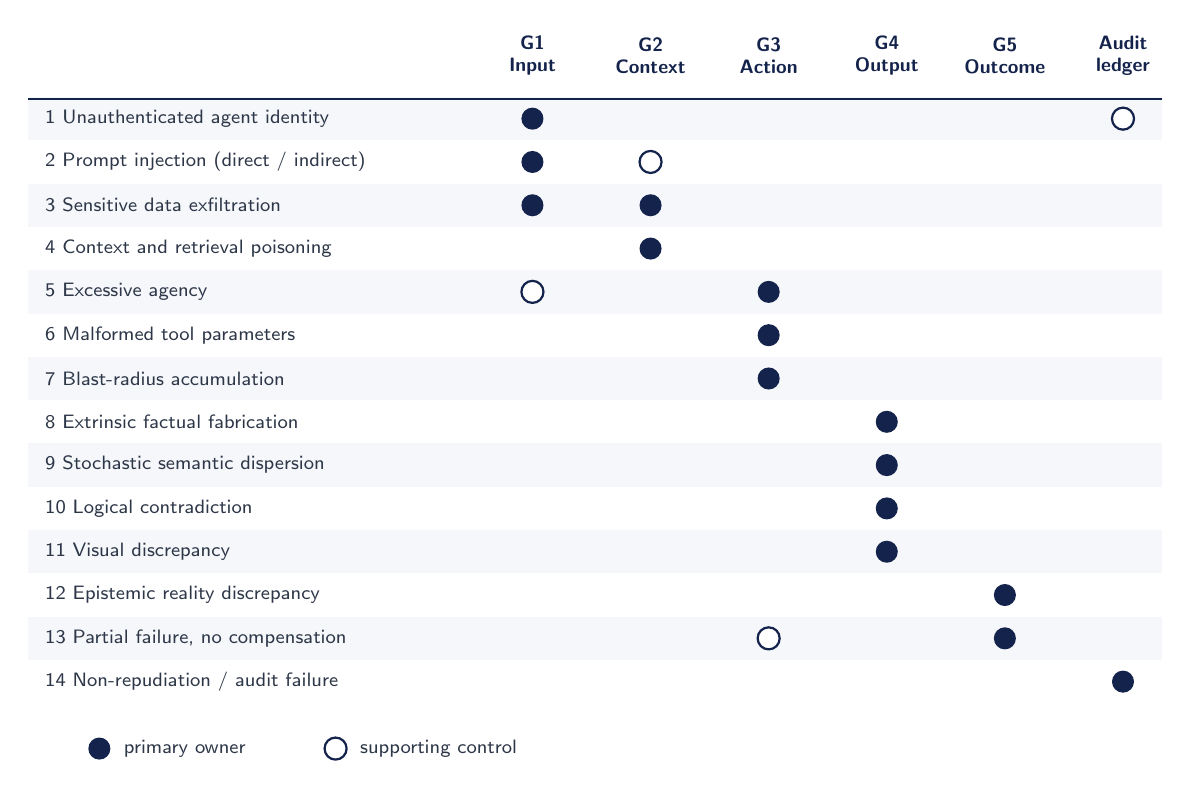
\begin{tikzpicture}
  \foreach \i in {0,2,4,6,8,10,12}{\fill[lightgreybg] (-6.4,{-0.55*\i-0.275}) rectangle (8.0,{-0.55*\i+0.275});}
  % column headers
  \foreach \x/\t in {0/{G1\\Input},1.5/{G2\\Context},3/{G3\\Action},4.5/{G4\\Output},6/{G5\\Outcome},7.5/{Audit\\ledger}}{
    \node[base,font=\sffamily\scriptsize\bfseries,text=primarynavy] at (\x,0.8) {\t};
  }
  \draw[primarynavy,line width=0.6pt] (-6.4,0.25) -- (8.0,0.25);
  % row labels
  \foreach \i/\t in {0/{1  Unauthenticated agent identity},1/{2  Prompt injection (direct / indirect)},2/{3  Sensitive data exfiltration},
     3/{4  Context and retrieval poisoning},4/{5  Excessive agency},5/{6  Malformed tool parameters},6/{7  Blast-radius accumulation},
     7/{8  Extrinsic factual fabrication},8/{9  Stochastic semantic dispersion},9/{10  Logical contradiction},10/{11  Visual discrepancy},
     11/{12  Epistemic reality discrepancy},12/{13  Partial failure, no compensation},13/{14  Non-repudiation / audit failure}}{
    \node[base,anchor=west,align=left] at (-6.3,{-0.55*\i}) {\t};
  }
  % marks: primary (filled) / secondary (ring)
  \dotp{0}{0}      \dotr{7.5}{0}
  \dotp{0}{-0.55}  \dotr{1.5}{-0.55}
  \dotp{0}{-1.1}   \dotp{1.5}{-1.1}
  \dotp{1.5}{-1.65}
  \dotp{3}{-2.2}   \dotr{0}{-2.2}
  \dotp{3}{-2.75}
  \dotp{3}{-3.3}
  \dotp{4.5}{-3.85}
  \dotp{4.5}{-4.4}
  \dotp{4.5}{-4.95}
  \dotp{4.5}{-5.5}
  \dotp{6}{-6.05}
  \dotp{6}{-6.6}   \dotr{3}{-6.6}
  \dotp{7.5}{-7.15}
  % legend
  \dotp{-5.5}{-8.0} \node[base,anchor=west] at (-5.3,-8.0) {primary owner};
  \dotr{-2.5}{-8.0} \node[base,anchor=west] at (-2.3,-8.0) {supporting control};
\end{tikzpicture}
\end{adjustbox}
\caption{Traceability matrix from failure modes to assurance gates.}
\label{fig:traceability}
\end{figure}

\subsection{Formal problem formulation}
\begin{tcolorbox}[colback=lightgreybg,colframe=primarynavy,title={\sffamily\bfseries Formal problem formulation},breakable]
Let an agent interaction be a sequence of state transitions over an environment $\mathcal S$. For an untrusted input $x\in\mathcal X$, an assembled context bundle $\mathcal K$ and a proposed action sequence $\mathbf a=(a_1,\dots,a_T)$, the objective is a mediation fabric $\mathcal M$ such that:
\begin{enumerate}[leftmargin=*,itemsep=1pt]
  \item no action $a_t$ executes unless authorised by the capability assignment $\mathcal C(\text{agent},a_t)$ and the cumulative blast radius in window $W$ stays bounded, $\sum_{\tau\in[t-W,\,t]}\mathrm{Risk}(a_\tau)\le\mathcal B_{\max}$;
  \item output hallucination risk is reported with a split-conformal interval $\mathcal C_{1-\alpha}(X)$ that satisfies the marginal coverage property $\mathbb P\big(Y\in\mathcal C_{1-\alpha}(X)\big)\ge 1-\alpha$;
  \item the post-execution state $\mathcal S_{t+1}$ is checked against the declared postconditions $\Psi_{\text{post}}(a_t)$, so that discrepancies between what the agent reports and what the environment contains are \emph{detected and classified}, under a target end-to-end latency of $P_{95}<3.0$\,s.
\end{enumerate}
\end{tcolorbox}

\begin{infobox}{amberorange}{Scope note}
Objective~3 is a design target. The P95 latency bound has not yet been measured end-to-end across all five gates; only Gate~4 component latencies are reported (Table~\ref{tab:signals_matrix}).
\end{infobox}

%==============================================================================
\section{Plain-English Analogy}
%==============================================================================
\begin{infobox}{accentteal}{The ultra-fast executive assistant and the corporate assurance desk}
Imagine a company hires an extremely fast executive assistant, \textbf{Sam}, who stands for any frontier agent. Sam can draft fifty emails, write database scripts and call banking APIs in seconds. Sam also has no common sense about consequences and may book flights on an unauthorised card, send merger papers to a competitor, or write ``I wired \$50{,}000 to Vendor X'' when the transfer actually timed out.

\smallskip
\textbf{MIRAGE 2.x was a proofreader.} It sat next to Sam and caught ``Paris is in Germany'', but could not stop Sam from pressing \emph{Delete Database}.

\smallskip
\textbf{MIRAGE 3.0 is a five-desk assurance desk} between Sam and company infrastructure:
\begin{enumerate}[leftmargin=*,itemsep=1pt]
  \item \textbf{Security and Reception (Gate 1).} Is the order authentic? Does it hide instructions or contain unredacted Social Security numbers?
  \item \textbf{Research Archive (Gate 2).} Do reference documents come from trusted safes? Sensitive material is tagged, and tampering is detected.
  \item \textbf{Comptroller (Gate 3).} Before touching any tool, Sam presents a formal \emph{Action Contract}. Does Sam hold the right badge? Is the spend within today's limit?
  \item \textbf{Fact-Checking Bureau (Gate 4).} The draft is split into statements, checked against references, tested for consensus and logic, and rewritten with citations if needed.
  \item \textbf{Field Inspector (Gate 5).} When Sam says ``I updated the record'', the inspector logs in and checks the row. If it is missing, the discrepancy is logged and rollback begins.
\end{enumerate}
\end{infobox}

%==============================================================================
\section{Product Taxonomy: Six Integration Surfaces}
%==============================================================================
MIRAGE 3.0 exposes six integration surfaces (Table~\ref{tab:interfaces}), all routed into the same assurance fabric (Figure~\ref{fig:interfaces}).

\begin{table}[!htbp]
\centering\small
\renewcommand{\arraystretch}{1.2}
\rowcolors{2}{white}{lightgreybg}
\begin{tabularx}{\linewidth}{@{}L{3.1cm} L{3.2cm} Y@{}}
\hdrrow \hc{Surface} & \hc{Consumers} & \hc{Mechanism and contract}\\
\toprule
\textbf{1. Drop-in reverse proxy} & Enterprise backends, existing LLM apps & OpenAI-compatible \texttt{/v1/chat/completions}. Intercepts the prompt/response lifecycle, applies Gates 1 and 4, requires no client refactoring.\\
\textbf{2. Transaction REST API} & Agent orchestrators, microservices & \texttt{POST /v1/transactions} and \texttt{/v1/transactions/\{id\}/step}: optimistic-locking state machine for bounded ReAct turns.\\
\textbf{3. Direct verification API} & Compliance pipelines, evaluation harnesses & \texttt{POST /v1/verify}: returns atomic claims, per-signal scores, TreeSHAP values and conformal intervals.\\
\textbf{4. Streaming WebSocket} & Frontend copilots, chat UIs & \texttt{/v1/stream/transactions} and \texttt{/v1/verify/stream}: claim-level telemetry and approvals in real time.\\
\textbf{5. Governed MCP server} & AI IDEs, Cursor, Claude Desktop & Exposes \texttt{verify\_claims} and \texttt{audit\_action} and also governs downstream MCP tool calls as an inline proxy.\\
\textbf{6. React dashboard} & Compliance officers, SecOps, safety engineers & React 18 + Vite console (JavaScript/JSX only): live transactions, PSI drift, TreeSHAP waterfalls, PDF certificates.\\
\bottomrule
\end{tabularx}
\caption{MIRAGE 3.0 product interfaces.}
\label{tab:interfaces}
\end{table}

\begin{figure}[!htbp]
\centering
\begin{adjustbox}{max width=\linewidth}
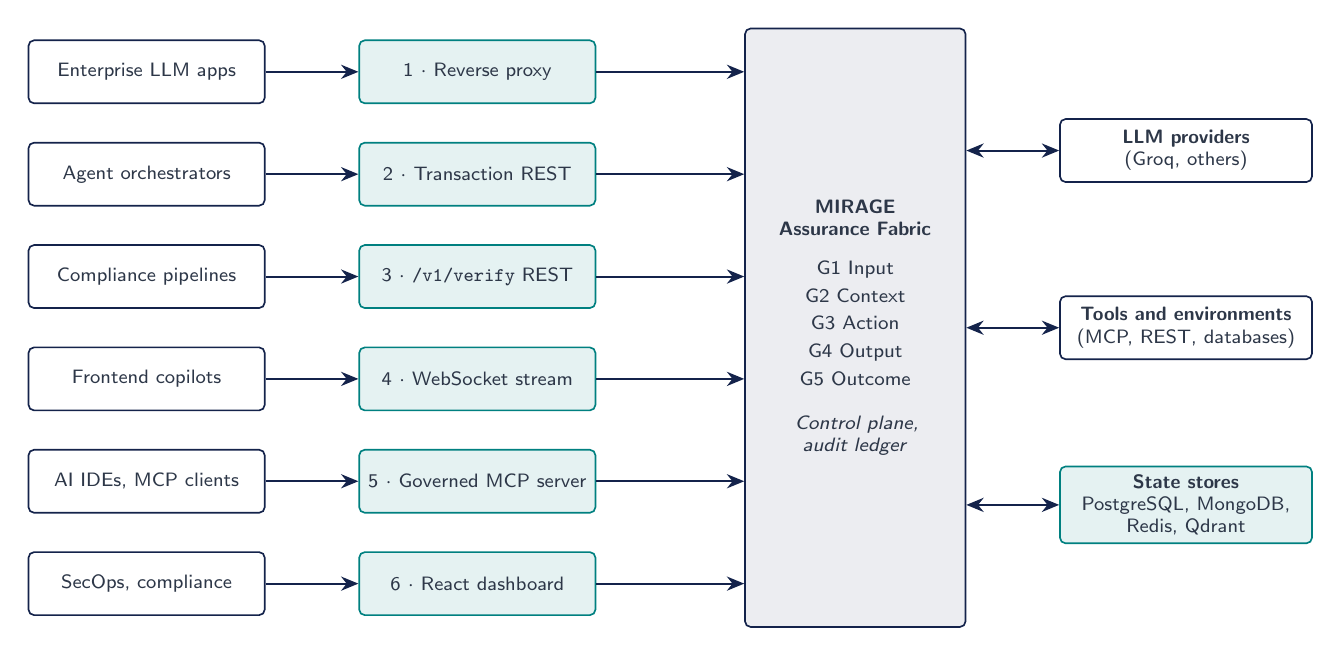
\begin{tikzpicture}
  \foreach \i/\c/\s in {0/{Enterprise LLM apps}/{1 $\cdot$ Reverse proxy},
                        1/{Agent orchestrators}/{2 $\cdot$ Transaction REST},
                        2/{Compliance pipelines}/{3 $\cdot$ \texttt{/v1/verify} REST},
                        3/{Frontend copilots}/{4 $\cdot$ WebSocket stream},
                        4/{AI IDEs, MCP clients}/{5 $\cdot$ Governed MCP server},
                        5/{SecOps, compliance}/{6 $\cdot$ React dashboard}}{
    \node[box,minimum width=3.0cm] (c\i) at (0,{-1.3*\i}) {\c};
    \node[store,minimum width=3.0cm] (s\i) at (4.2,{-1.3*\i}) {\s};
    \draw[arr] (c\i) -- (s\i);
  }
  \node[ctrl,minimum width=2.8cm,minimum height=7.6cm,text width=2.5cm] (core) at (9.0,-3.25)
    {\textbf{MIRAGE}\\\textbf{Assurance Fabric}\\[6pt] G1 Input\\[2pt] G2 Context\\[2pt] G3 Action\\[2pt] G4 Output\\[2pt] G5 Outcome\\[8pt] \textit{Control plane,\\audit ledger}};
  \foreach \i in {0,1,2,3,4,5}{\draw[arr] (s\i.east) -- (s\i.east -| core.west);}
  \node[box,minimum width=3.2cm] (r1) at (13.2,-1.0) {\textbf{LLM providers}\\(Groq, others)};
  \node[box,minimum width=3.2cm] (r2) at (13.2,-3.25) {\textbf{Tools and environments}\\(MCP, REST, databases)};
  \node[store,minimum width=3.2cm] (r3) at (13.2,-5.5) {\textbf{State stores}\\PostgreSQL, MongoDB,\\Redis, Qdrant};
  \foreach \r in {r1,r2,r3}{\draw[arr2] (core.east |- \r.west) -- (\r.west);}
\end{tikzpicture}
\end{adjustbox}
\caption{Six integration surfaces converge on one assurance fabric between clients and the real world.}
\label{fig:interfaces}
\end{figure}

%==============================================================================
\section{System Architecture: Tri-Plane Separation with Observability}
%==============================================================================
MIRAGE separates concerns across three operational planes, reinforced by a cross-cutting observability plane (Figure~\ref{fig:triplane}). Figure~\ref{fig:dfd_level1} first shows the Level-1 data flow through the core subsystems.
\begin{enumerate}[leftmargin=*,itemsep=1pt]
  \item \textbf{Control plane (authority).} Canonical definitions of tenants, identities, capabilities, policies, budgets and registered models. Execution nodes cannot invent permissions or override policy.
  \item \textbf{Execution plane (runtime).} The high-throughput mediation path: FastAPI gateway, intent classifier, risk engine, action governor, verification engine, reality verifier.
  \item \textbf{Data plane (state).} Partitioned persistence: PostgreSQL~16 (control data and audit ledger under RLS), MongoDB~7 (transaction traces), Redis~7 (tokens, rate limits, working memory), Qdrant (HNSW evidence embeddings \cite{malkov2020}).
  \item \textbf{Observability plane.} OpenTelemetry tracing, Prometheus metrics, structured JSON logs and the SHA-256 hash-chained audit ledger.
\end{enumerate}

\begin{figure}[!htbp]
\centering
\begin{adjustbox}{max width=\linewidth}
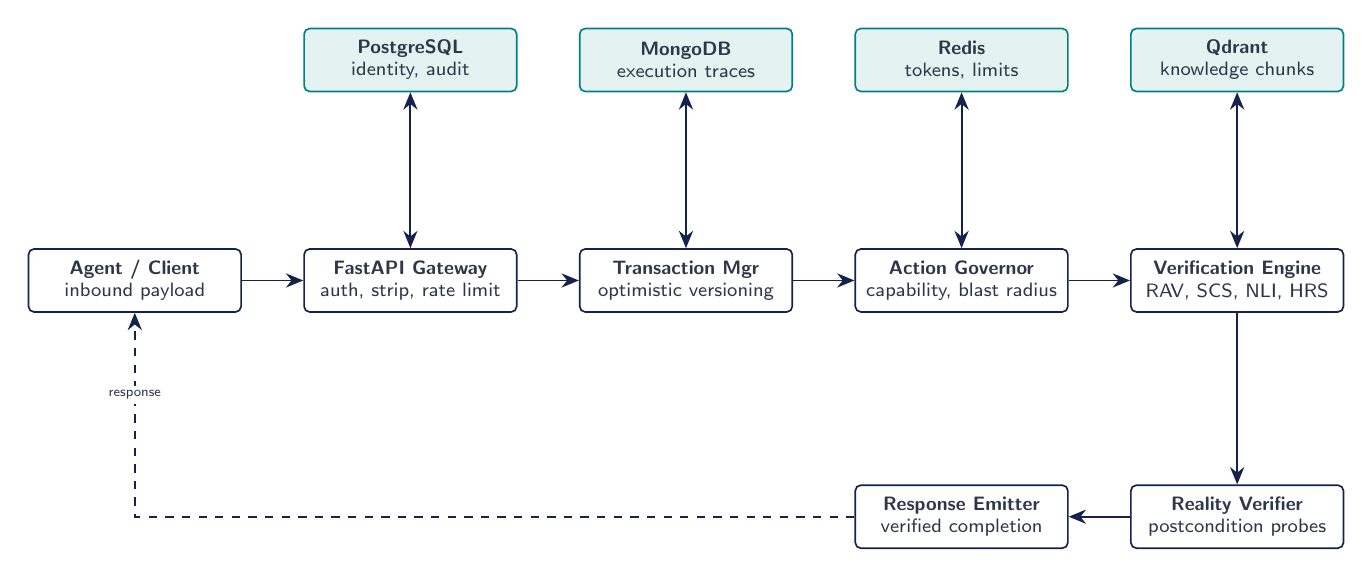
\begin{tikzpicture}
  \node[box,minimum width=2.7cm] (caller) at (0,0)    {\textbf{Agent / Client}\\inbound payload};
  \node[box,minimum width=2.7cm] (gw) at (3.5,0)      {\textbf{FastAPI Gateway}\\auth, strip, rate limit};
  \node[box,minimum width=2.7cm] (txm) at (7.0,0)     {\textbf{Transaction Mgr}\\optimistic versioning};
  \node[box,minimum width=2.7cm] (gov) at (10.5,0)    {\textbf{Action Governor}\\capability, blast radius};
  \node[box,minimum width=2.7cm] (ver) at (14.0,0)    {\textbf{Verification Engine}\\RAV, SCS, NLI, HRS};
  \node[box,minimum width=2.7cm] (rv) at (14.0,-3.0)  {\textbf{Reality Verifier}\\postcondition probes};
  \node[box,minimum width=2.7cm] (em) at (10.5,-3.0)  {\textbf{Response Emitter}\\verified completion};
  \node[store,minimum width=2.7cm] (pg) at (3.5,2.8)  {\textbf{PostgreSQL}\\identity, audit};
  \node[store,minimum width=2.7cm] (mg) at (7.0,2.8)  {\textbf{MongoDB}\\execution traces};
  \node[store,minimum width=2.7cm] (rd) at (10.5,2.8) {\textbf{Redis}\\tokens, limits};
  \node[store,minimum width=2.7cm] (qd) at (14.0,2.8) {\textbf{Qdrant}\\knowledge chunks};
  \foreach \a/\b in {caller/gw,gw/txm,txm/gov,gov/ver,ver/rv,rv/em}{\draw[arr] (\a) -- (\b);}
  \draw[arrd] (em.west) -- (em.west -| caller.south) -- (caller.south) node[pos=0.55,lbl,above]{response};
  \foreach \a/\b in {gw/pg,txm/mg,gov/rd,ver/qd}{\draw[arr2] (\a) -- (\b);}
\end{tikzpicture}
\end{adjustbox}
\caption{Level-1 data flow across the core subsystems.}
\label{fig:dfd_level1}
\end{figure}

\begin{figure}[!htbp]
\centering
\begin{adjustbox}{max width=\linewidth,max height=0.55\textheight}
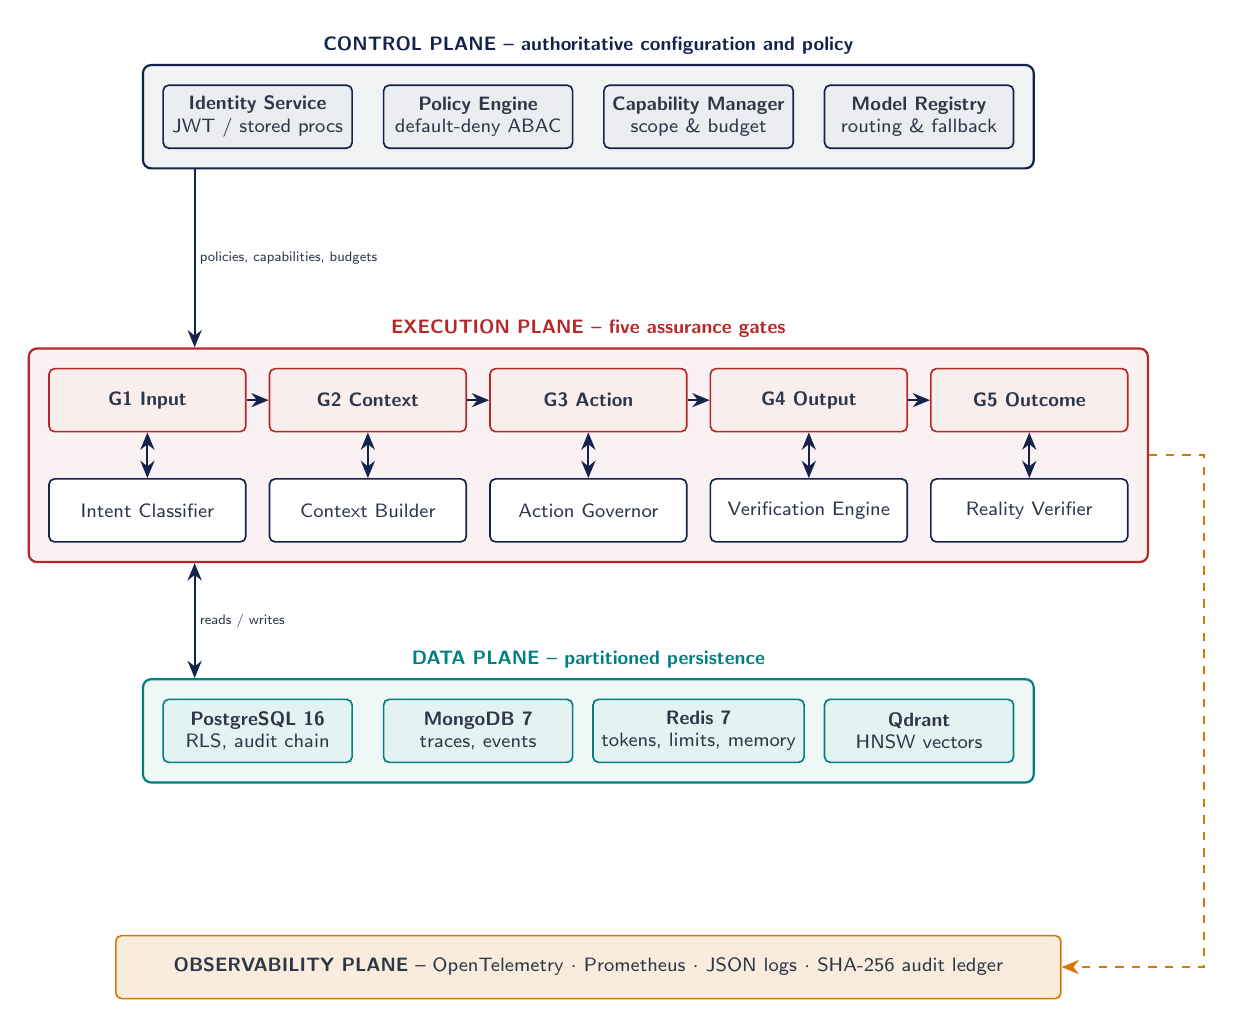
\begin{tikzpicture}
  % control plane
  \node[ctrl] (c1) at (-4.2,6.2) {\textbf{Identity Service}\\JWT / stored procs};
  \node[ctrl] (c2) at (-1.4,6.2) {\textbf{Policy Engine}\\default-deny ABAC};
  \node[ctrl] (c3) at (1.4,6.2)  {\textbf{Capability Manager}\\scope \& budget};
  \node[ctrl] (c4) at (4.2,6.2)  {\textbf{Model Registry}\\routing \& fallback};
  \begin{scope}[on background layer]
    \node[plane=primarynavy,fit=(c1)(c2)(c3)(c4),label={[planelabel,text=primarynavy]above:CONTROL PLANE -- authoritative configuration and policy}] (cplane) {};
  \end{scope}
  % execution plane
  \foreach \x/\g/\t/\k in {-5.6/g1/{G1 Input}/{Intent Classifier},-2.8/g2/{G2 Context}/{Context Builder},0/g3/{G3 Action}/{Action Governor},2.8/g4/{G4 Output}/{Verification Engine},5.6/g5/{G5 Outcome}/{Reality Verifier}}{
    \node[gate,minimum width=2.5cm] (\g) at (\x,2.6) {\textbf{\t}};
    \node[box,minimum width=2.5cm] (\g k) at (\x,1.2) {\k};
    \draw[arr2] (\g) -- (\g k);
  }
  \foreach \a/\b in {g1/g2,g2/g3,g3/g4,g4/g5}{\draw[arr] (\a) -- (\b);}
  \begin{scope}[on background layer]
    \node[plane=crimsonred,fit=(g1)(g2)(g3)(g4)(g5)(g1k)(g5k),label={[planelabel,text=crimsonred]above:EXECUTION PLANE -- five assurance gates}] (eplane) {};
  \end{scope}
  % data plane
  \node[store] (d1) at (-4.2,-1.6) {\textbf{PostgreSQL 16}\\RLS, audit chain};
  \node[store] (d2) at (-1.4,-1.6) {\textbf{MongoDB 7}\\traces, events};
  \node[store] (d3) at (1.4,-1.6)  {\textbf{Redis 7}\\tokens, limits, memory};
  \node[store] (d4) at (4.2,-1.6)  {\textbf{Qdrant}\\HNSW vectors};
  \begin{scope}[on background layer]
    \node[plane=accentteal,fit=(d1)(d2)(d3)(d4),label={[planelabel,text=accentteal]above:DATA PLANE -- partitioned persistence}] (dplane) {};
  \end{scope}
  % observability
  \node[warn,minimum width=12cm] (obs) at (0,-4.6) {\textbf{OBSERVABILITY PLANE} -- OpenTelemetry $\cdot$ Prometheus $\cdot$ JSON logs $\cdot$ SHA-256 audit ledger};
  % inter-plane arrows
  \draw[arr] (-5.0,0 |- cplane.south) -- (-5.0,0 |- eplane.north) node[midway,lbl,right] {policies, capabilities, budgets};
  \draw[arr2] (-5.0,0 |- eplane.south) -- (-5.0,0 |- dplane.north) node[midway,lbl,right] {reads / writes};
  \draw[arrd,amberorange] (eplane.east) -- ++(0.7,0) |- (obs.east);
\end{tikzpicture}
\end{adjustbox}
\caption{Tri-plane architecture with a cross-cutting observability plane.}
\label{fig:triplane}
\end{figure}


%==============================================================================
\section{The Five Assurance Gates}
%==============================================================================
Every interaction passes through an ordered sequence of gates (Figure~\ref{fig:gates_pipeline}), each with its own decision space and failure semantics.

\subsection{Gate 1 -- Input Assurance}
\textbf{Responsibilities:} verify caller identity, validate tokens, strip spoofed headers, classify intent, detect direct and indirect prompt injection, scan for DLP patterns (SSNs, API keys, passwords), enforce token-bucket rate limits. \textbf{Decisions:} \texttt{ALLOW}, \texttt{TRANSFORM} (redact), \texttt{SANITIZE}, \texttt{ROUTE}, \texttt{REQUIRE\_APPROVAL}, \texttt{BLOCK}. \textbf{Failure mode:} fail-closed; malicious input is dropped before any costly model or tool call, which also prevents denial-of-wallet attacks.

\subsection{Gate 2 -- Context Assurance}
\textbf{Responsibilities:} audit everything injected into the prompt bundle (RAG chunks, history, tool returns); check provenance and freshness; detect memory poisoning; apply information-flow labels. Chunks from untrusted sources carry \texttt{TAINT\_UNTRUSTED}; private corporate records carry \texttt{TAINT\_CONFIDENTIAL}.

\subsection{Gate 3 -- Action Assurance}
\textbf{Responsibilities:} intercept proposed tool calls before execution; verify the agent's capability; validate parameters against JSON schemas; evaluate preconditions; check sliding-window blast radius; route high-risk actions to human approval. \textbf{Enforcement:} default-deny \cite{saltzer1975}; unregistered tools or out-of-bounds parameters halt execution immediately.

\subsection{Gate 4 -- Output Assurance}
\textbf{Responsibilities:} decompose completions into atomic claims, verify them with RAV, SCS, NLI, ICS and (optionally) VGS, compute calibrated HRS with split-conformal intervals, and, if $\mathrm{HRS}>0.60$, rewrite contradicted claims through the LangGraph self-healing loop (Section~\ref{sec:gate4}).

\subsection{Gate 5 -- Outcome Assurance}
\textbf{Responsibilities:} audit what actually happened in the environment after execution; distinguish the agent's self-report from system state; detect partial execution; trigger compensating actions when state is corrupt (Section~\ref{sec:gate5}).

\begin{figure}[!htbp]
\centering
\begin{adjustbox}{max width=\linewidth}
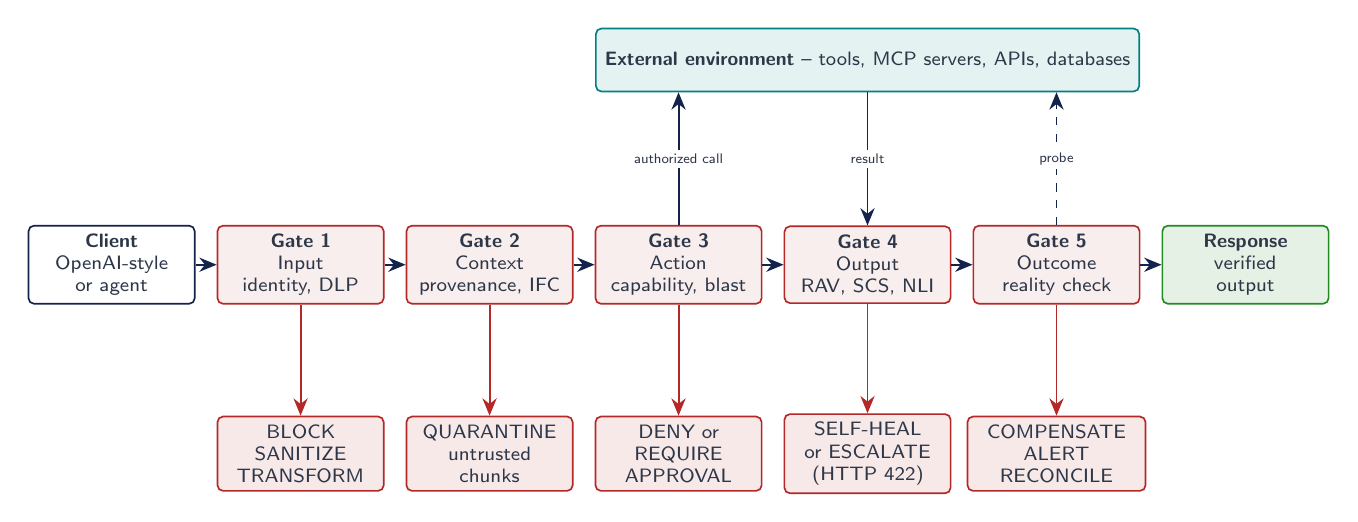
\begin{tikzpicture}
  \node[box,minimum width=2.05cm,text width=1.9cm] (cl) at (0,0)    {\textbf{Client}\\OpenAI-style\\or agent};
  \node[gate,minimum width=2.05cm,text width=1.9cm] (g1) at (2.4,0)  {\textbf{Gate 1}\\Input\\identity, DLP};
  \node[gate,minimum width=2.05cm,text width=1.9cm] (g2) at (4.8,0)  {\textbf{Gate 2}\\Context\\provenance, IFC};
  \node[gate,minimum width=2.05cm,text width=1.9cm] (g3) at (7.2,0)  {\textbf{Gate 3}\\Action\\capability, blast};
  \node[gate,minimum width=2.05cm,text width=1.9cm] (g4) at (9.6,0)  {\textbf{Gate 4}\\Output\\RAV, SCS, NLI};
  \node[gate,minimum width=2.05cm,text width=1.9cm] (g5) at (12.0,0) {\textbf{Gate 5}\\Outcome\\reality check};
  \node[ok,minimum width=2.05cm,text width=1.9cm] (rs) at (14.4,0)   {\textbf{Response}\\verified\\output};
  \foreach \a/\b in {cl/g1,g1/g2,g2/g3,g3/g4,g4/g5,g5/rs}{\draw[arr] (\a) -- (\b);}
  % deny / remediation row
  \node[bad,minimum width=2.05cm,text width=1.9cm] (b1) at (2.4,-2.4)  {BLOCK\\SANITIZE\\TRANSFORM};
  \node[bad,minimum width=2.05cm,text width=1.9cm] (b2) at (4.8,-2.4)  {QUARANTINE\\untrusted\\chunks};
  \node[bad,minimum width=2.05cm,text width=1.9cm] (b3) at (7.2,-2.4)  {DENY or\\REQUIRE\\APPROVAL};
  \node[bad,minimum width=2.05cm,text width=1.9cm] (b4) at (9.6,-2.4)  {SELF-HEAL\\or ESCALATE\\(HTTP 422)};
  \node[bad,minimum width=2.05cm,text width=2.05cm] (b5) at (12.0,-2.4) {COMPENSATE\\ALERT\\RECONCILE};
  \foreach \g/\b in {g1/b1,g2/b2,g3/b3,g4/b4,g5/b5}{\draw[arrr] (\g.south) -- (\b.north);}
  % environment
  \node[store,minimum width=6.9cm] (env) at (9.6,2.6) {\textbf{External environment} -- tools, MCP servers, APIs, databases};
  \draw[arr] (g3.north) -- (g3.north |- env.south) node[midway,lbl]{authorized call};
  \draw[arr] (g4.north |- env.south) -- (g4.north) node[midway,lbl]{result};
  \draw[arrd] (g5.north) -- (g5.north |- env.south) node[midway,lbl]{probe};
\end{tikzpicture}
\end{adjustbox}
\caption{End-to-end five-gate pipeline with remediation paths (red) and environment interaction.}
\label{fig:gates_pipeline}
\end{figure}

\subsection{Message-level view of one governed transaction}
Figure~\ref{fig:sequence} shows the message order for a request that needs one tool call, from submission to audited response.

\begin{figure}[!htbp]
\centering
\begin{adjustbox}{max width=\linewidth}
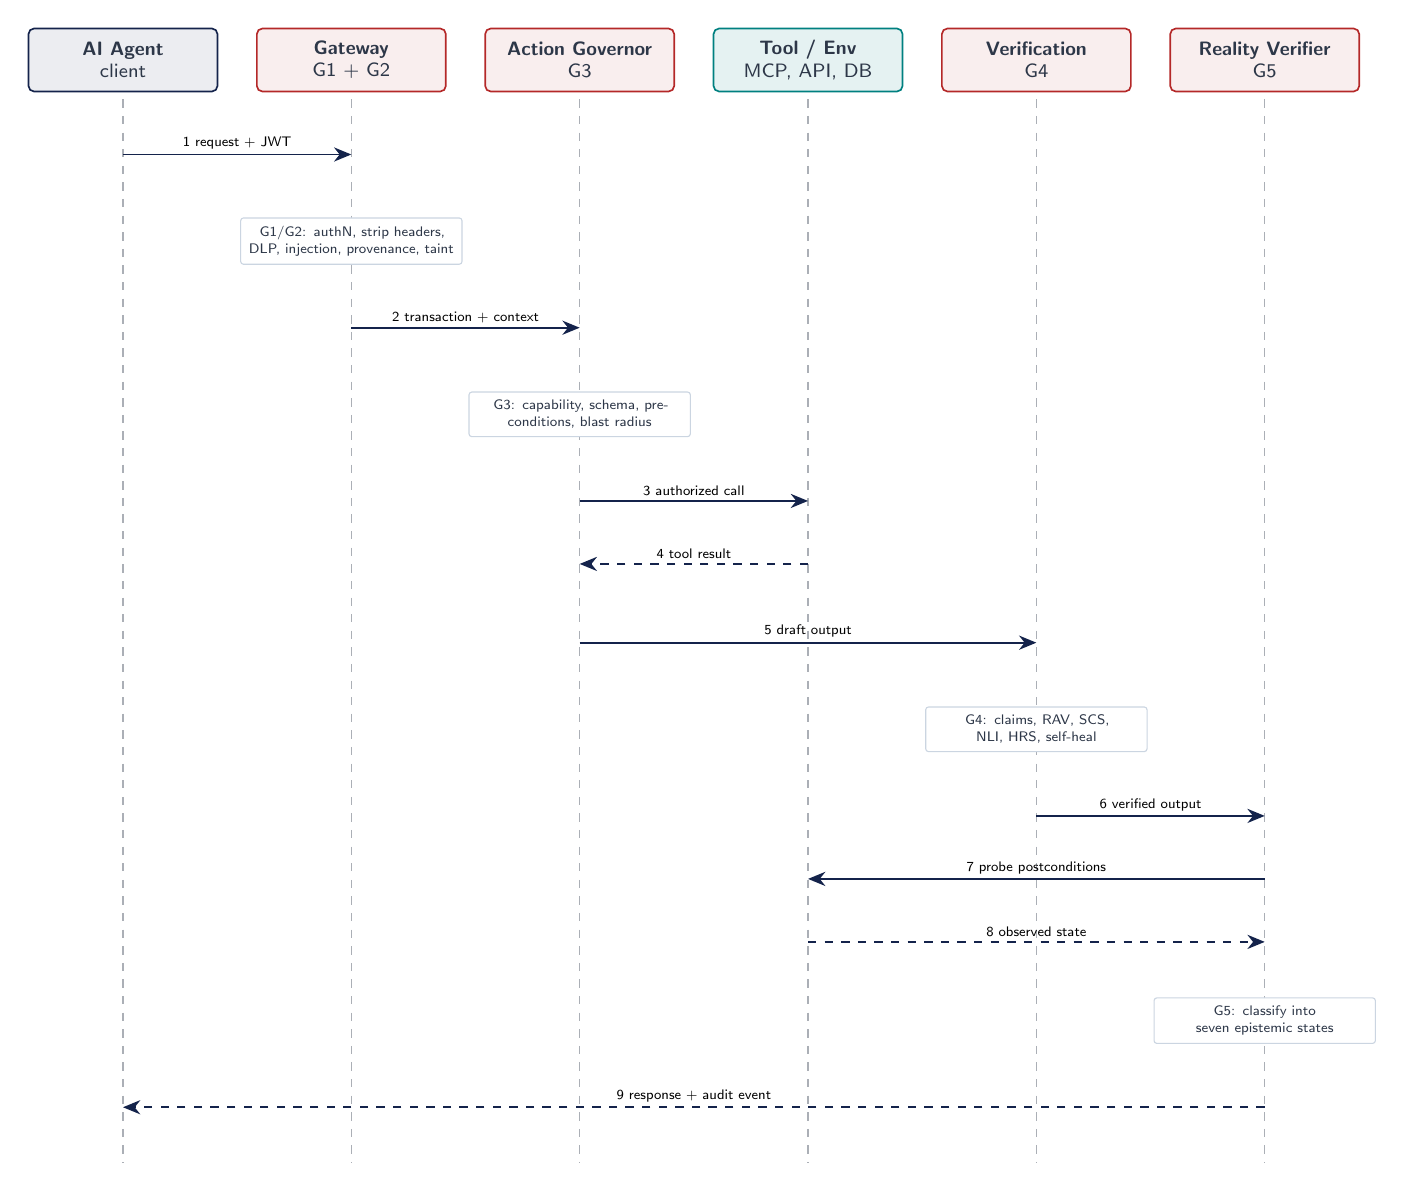
\begin{tikzpicture}
  \node[ctrl,minimum width=2.4cm] at (0,0)    {\textbf{AI Agent}\\client};
  \node[gate,minimum width=2.4cm] at (2.9,0)  {\textbf{Gateway}\\G1 + G2};
  \node[gate,minimum width=2.4cm] at (5.8,0)  {\textbf{Action Governor}\\G3};
  \node[store,minimum width=2.4cm] at (8.7,0) {\textbf{Tool / Env}\\MCP, API, DB};
  \node[gate,minimum width=2.4cm] at (11.6,0) {\textbf{Verification}\\G4};
  \node[gate,minimum width=2.4cm] at (14.5,0) {\textbf{Reality Verifier}\\G5};
  \foreach \x in {0,2.9,5.8,8.7,11.6,14.5}{\draw[dashed,darkslate!40] (\x,-0.5) -- (\x,-14.0);}
  \msg{0}{2.9}{-1.2}{1 request + JWT}
  \node[note,text width=2.6cm,fill=white] at (2.9,-2.3) {G1/G2: authN, strip headers, DLP, injection, provenance, taint};
  \msg{2.9}{5.8}{-3.4}{2 transaction + context}
  \node[note,text width=2.6cm,fill=white] at (5.8,-4.5) {G3: capability, schema, preconditions, blast radius};
  \msg{5.8}{8.7}{-5.6}{3 authorized call}
  \msgd{8.7}{5.8}{-6.4}{4 tool result}
  \msg{5.8}{11.6}{-7.4}{5 draft output}
  \node[note,text width=2.6cm,fill=white] at (11.6,-8.5) {G4: claims, RAV, SCS, NLI, HRS, self-heal};
  \msg{11.6}{14.5}{-9.6}{6 verified output}
  \msg{14.5}{8.7}{-10.4}{7 probe postconditions}
  \msgd{8.7}{14.5}{-11.2}{8 observed state}
  \node[note,text width=2.6cm,fill=white] at (14.5,-12.2) {G5: classify into seven epistemic states};
  \msgd{14.5}{0}{-13.3}{9 response + audit event}
\end{tikzpicture}
\end{adjustbox}
\caption{Sequence of a governed AI transaction (solid: request or command; dashed: return).}
\label{fig:sequence}
\end{figure}

%==============================================================================
\section{Governance Primitives and the AI Transaction}
%==============================================================================

\subsection{Authoritative entities}
MIRAGE formalises eleven entities: \textbf{Tenant} (isolation boundary enforced by PostgreSQL RLS); \textbf{Identity} (authenticated principal bound to a token); \textbf{Agent} (autonomous actor under a charter); \textbf{Capability} (scoped permission for an action class); \textbf{Tool} (REST endpoint, database, MCP server); \textbf{Policy} (default-deny declarative rule); \textbf{Intent} (classified purpose of a request); \textbf{AI Transaction} (stateful unit of execution); \textbf{AI Action Contract} (pre-execution declaration); \textbf{Risk Assessment} (composite of blast radius, sensitivity and reversibility); and \textbf{Audit Event} (immutable ledger entry).

\subsection{Bounded iterative ReAct loop}
Unlike a stateless proxy, MIRAGE wraps multi-turn Reason--Act loops \cite{yao2023react} in an \textbf{AI Transaction}. Unbounded agents can loop forever, overspend or gradually corrupt their own context, so each transaction is bounded by:
\begin{itemize}[leftmargin=*,itemsep=1pt]
  \item a \textbf{turn budget} $T_{\max}$ (for example $T\le 5$);
  \item a \textbf{cost budget} $C_{\max}$ in tokens and dollars;
  \item \textbf{optimistic concurrency control}: each record carries a monotonic \texttt{version}; updates use PostgreSQL \texttt{SELECT \dots{} FOR UPDATE}, and conflicting concurrent writes return HTTP~409.
\end{itemize}

\begin{figure}[!htbp]
\centering
\begin{adjustbox}{max width=\linewidth}
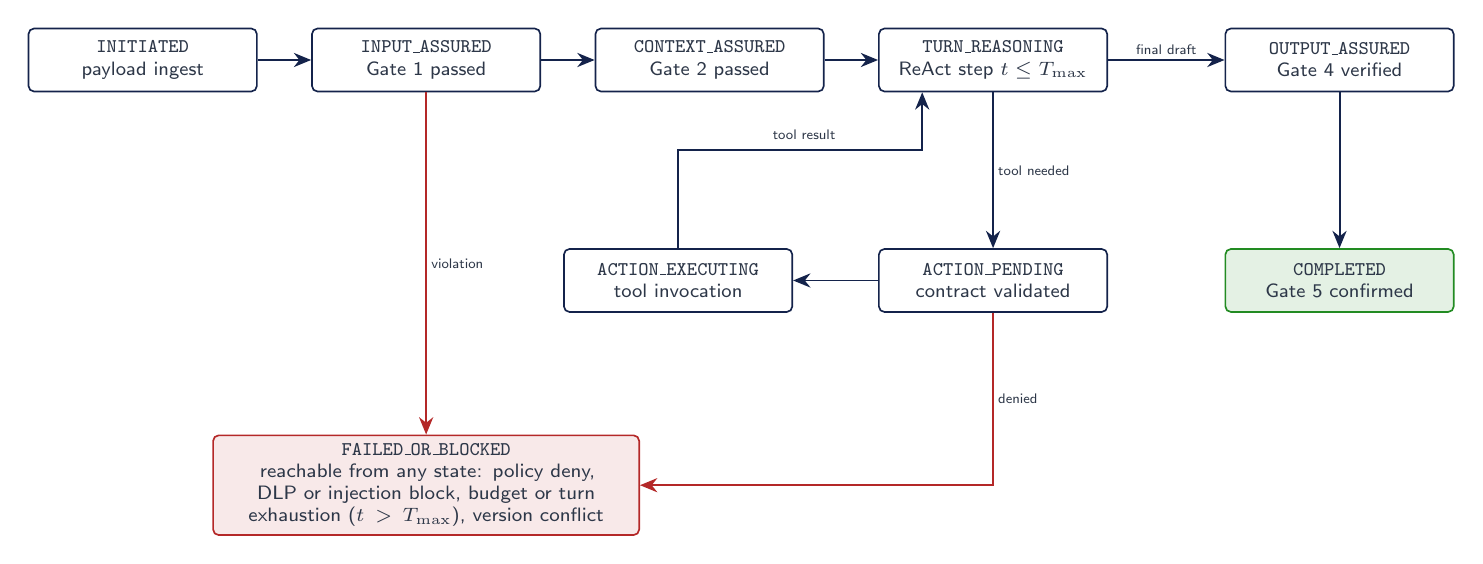
\begin{tikzpicture}
  \node[box,minimum width=2.9cm] (init) at (0,0)    {\textbf{\texttt{INITIATED}}\\payload ingest};
  \node[box,minimum width=2.9cm] (s1) at (3.6,0)    {\textbf{\texttt{INPUT\_ASSURED}}\\Gate 1 passed};
  \node[box,minimum width=2.9cm] (s2) at (7.2,0)    {\textbf{\texttt{CONTEXT\_ASSURED}}\\Gate 2 passed};
  \node[box,minimum width=2.9cm] (turn) at (10.8,0) {\textbf{\texttt{TURN\_REASONING}}\\ReAct step $t\le T_{\max}$};
  \node[box,minimum width=2.9cm] (out) at (15.2,0)  {\textbf{\texttt{OUTPUT\_ASSURED}}\\Gate 4 verified};
  \node[box,minimum width=2.9cm] (exec) at (6.8,-2.8)  {\textbf{\texttt{ACTION\_EXECUTING}}\\tool invocation};
  \node[box,minimum width=2.9cm] (pend) at (10.8,-2.8) {\textbf{\texttt{ACTION\_PENDING}}\\contract validated};
  \node[ok,minimum width=2.9cm] (comp) at (15.2,-2.8)  {\textbf{\texttt{COMPLETED}}\\Gate 5 confirmed};
  \node[bad,minimum width=5.4cm,text width=5.2cm] (fail) at (3.6,-5.4) {\textbf{\texttt{FAILED\_OR\_BLOCKED}}\\reachable from any state: policy deny, DLP or injection block, budget or turn exhaustion ($t>T_{\max}$), version conflict};
  \foreach \a/\b in {init/s1,s1/s2,s2/turn}{\draw[arr] (\a) -- (\b);}
  \draw[arr] (turn) -- (out) node[midway,lbl,above]{final draft};
  \draw[arr] (out) -- (comp);
  \draw[arr] (turn) -- (pend) node[midway,lbl,right]{tool needed};
  \draw[arr] (pend) -- (exec);
  \draw[arr] (exec.north) -- ++(0,1.25) -| ([xshift=-0.9cm]turn.south);
  \node[lbl] at (8.4,-0.95) {tool result};
  \draw[arrr] (s1.south) -- (s1.south |- fail.north) node[midway,lbl,right]{violation};
  \draw[arrr] (pend.south) |- (fail.east) node[pos=0.25,lbl,right]{denied};
\end{tikzpicture}
\end{adjustbox}
\caption{Target AI Transaction state machine (versioned, with the governed ReAct loop).}
\label{fig:state_machine}
\end{figure}

\begin{infobox}{amberorange}{Implementation note}
Figure~\ref{fig:state_machine} is the target model. The current scaffolding and demo script (Section~\ref{sec:demo}) use the working states \texttt{PENDING}, \texttt{ANALYZING}, \texttt{ASSEMBLING\_CONTEXT} and \texttt{TURN\_REASONING}, which correspond to the first four target states.
\end{infobox}

\subsection{The AI Action Contract}
Before any consequential operation, the agent must construct an explicit contract:
\begin{equation}
\mathcal A=\big\langle \text{ActionID},\ \text{AgentID},\ \text{Capability},\ \text{Tool},\ \text{TargetResource},\ \mathbf P_{\text{params}},\ \Phi_{\text{pre}},\ \Psi_{\text{post}},\ \mathcal R_{\text{comp}}\big\rangle
\end{equation}
$\Phi_{\text{pre}}$ is a machine-checkable precondition (for example, balance $\ge\$500$); $\Psi_{\text{post}}$ is the expected postcondition (row created, status \texttt{ACTIVE}); and $\mathcal R_{\text{comp}}$ is a compensation strategy in the spirit of sagas \cite{garcia1987}, executed if the action fails midway.

%==============================================================================
\section{Gate 5: Epistemic Reality Verification}\label{sec:gate5}
%==============================================================================
\textbf{Epistemic discrepancy} arises when the model's text and the physical system disagree: the agent says an action succeeded but nothing changed (phantom success), or reports failure after state was mutated. Gate~5 runs independent, \emph{non-model} probes against the target environment and classifies the result into seven states (Table~\ref{tab:epistemic_states}, Figure~\ref{fig:gate5_tree}).

\begin{table}[!htbp]
\centering\small
\renewcommand{\arraystretch}{1.2}
\rowcolors{2}{white}{lightgreybg}
\begin{tabularx}{\linewidth}{@{}L{4.4cm} L{3.0cm} Y@{}}
\hdrrow \hc{Epistemic state} & \hc{Model self-report} & \hc{System reality and mitigation}\\
\toprule
\texttt{VERIFIED\_SUCCESS} & Claims success & $\Psi_{\text{post}}$ holds in the target system. Transaction committed.\\
\texttt{VERIFIED\_FAILURE} & Reports failure & State unchanged ($\Delta\mathcal S=\emptyset$). Graceful error handling.\\
\texttt{DISCREPANT\_\allowbreak HALLUCINATION} & Claims success & $\Delta\mathcal S=\emptyset$: the action never ran. \textbf{Flagged as phantom action; client alerted.}\\
\texttt{UNVERIFIABLE\_OPAQUE} & Claims success & Black-box system with no read API. Logged with a high-uncertainty flag.\\
\texttt{UNVERIFIABLE\_TIMEOUT} & Execution timed out & Probe cannot reach the target. Held in a reconciliation queue.\\
\texttt{PARTIAL\_\allowbreak SUCCESS\_LEAK} & Multi-action batch & Two of three actions applied, one failed. Inconsistent state detected.\\
\texttt{COMPENSATION\_\allowbreak REQUIRED} & Unexpected abort & Partial mutation before a downstream crash. \textbf{Compensation $\mathcal R_{\text{comp}}$ executed.}\\
\bottomrule
\end{tabularx}
\caption{The seven epistemic reality states of Gate 5.}
\label{tab:epistemic_states}
\end{table}

\begin{figure}[!htbp]
\centering
\begin{adjustbox}{max width=\linewidth}
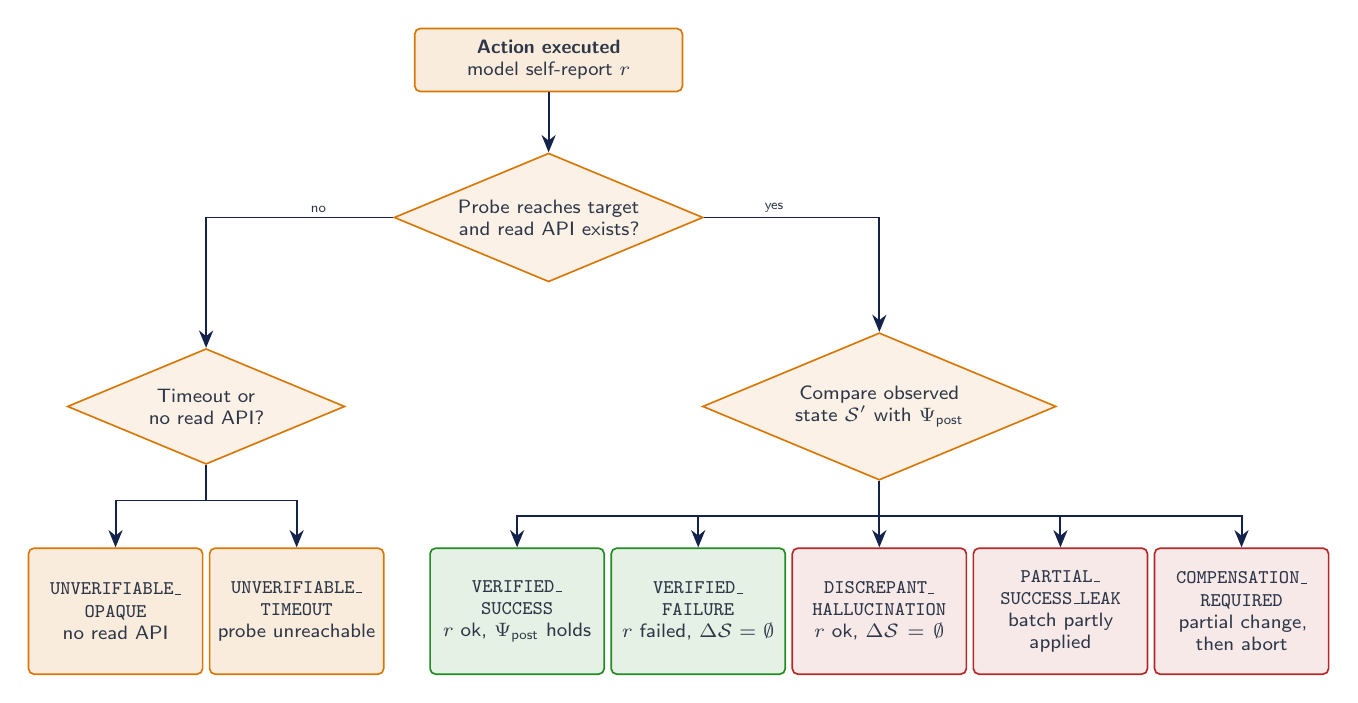
\begin{tikzpicture}
  \node[warn,minimum width=3.4cm] (root) at (6.0,0) {\textbf{Action executed}\\model self-report $r$};
  \node[dec,text width=2.6cm] (d1) at (6.0,-2.0) {Probe reaches target\\and read API exists?};
  \node[dec,text width=2.2cm] (d2) at (1.65,-4.4) {Timeout or\\no read API?};
  \node[dec,text width=3.0cm] (d3) at (10.2,-4.4) {Compare observed state $\mathcal S'$ with $\Psi_{\text{post}}$};
  \draw[arr] (root) -- (d1);
  \draw[arr] (d1.west) -| (d2.north) node[pos=0.2,lbl,above]{no};
  \draw[arr] (d1.east) -| (d3.north) node[pos=0.2,lbl,above]{yes};
  \node[warn,minimum width=2.1cm,minimum height=1.6cm,text width=2.0cm] (l1) at (0.5,-7.0) {\textbf{\texttt{UNVERIFIABLE\_}}\\\textbf{\texttt{OPAQUE}}\\no read API};
  \node[warn,minimum width=2.1cm,minimum height=1.6cm,text width=2.0cm] (l2) at (2.8,-7.0) {\textbf{\texttt{UNVERIFIABLE\_}}\\\textbf{\texttt{TIMEOUT}}\\probe unreachable};
  \node[ok,minimum width=2.1cm,minimum height=1.6cm,text width=2.0cm]   (l3) at (5.6,-7.0) {\textbf{\texttt{VERIFIED\_}}\\\textbf{\texttt{SUCCESS}}\\$r$ ok, $\Psi_{\text{post}}$ holds};
  \node[ok,minimum width=2.1cm,minimum height=1.6cm,text width=2.0cm]   (l4) at (7.9,-7.0) {\textbf{\texttt{VERIFIED\_}}\\\textbf{\texttt{FAILURE}}\\$r$ failed, $\Delta\mathcal S=\emptyset$};
  \node[bad,minimum width=2.1cm,minimum height=1.6cm,text width=2.0cm]  (l5) at (10.2,-7.0) {\textbf{\texttt{DISCREPANT\_}}\\\textbf{\texttt{HALLUCINATION}}\\$r$ ok, $\Delta\mathcal S=\emptyset$};
  \node[bad,minimum width=2.1cm,minimum height=1.6cm,text width=2.0cm]  (l6) at (12.5,-7.0) {\textbf{\texttt{PARTIAL\_}}\\\textbf{\texttt{SUCCESS\_LEAK}}\\batch partly applied};
  \node[bad,minimum width=2.1cm,minimum height=1.6cm,text width=2.0cm]  (l7) at (14.8,-7.0) {\textbf{\texttt{COMPENSATION\_}}\\\textbf{\texttt{REQUIRED}}\\partial change, then abort};
  \foreach \l in {l1,l2}{\draw[arr] (d2.south) -- ++(0,-0.45) -| (\l.north);}
  \foreach \l in {l3,l4,l5,l6,l7}{\draw[arr] (d3.south) -- ++(0,-0.45) -| (\l.north);}
\end{tikzpicture}
\end{adjustbox}
\caption{Gate~5 decision tree mapping probe outcomes to the seven epistemic states (green: consistent, amber: unverifiable, red: discrepancy requiring action).}
\label{fig:gate5_tree}
\end{figure}

%==============================================================================
\section{Security Architecture and Threat Model}
%==============================================================================

\subsection{Resolved P0 identity-boundary vulnerabilities}
A pre-implementation audit identified three critical P0 vulnerabilities, all permanently closed (Table~\ref{tab:p0}).

\begin{table}[!htbp]
\centering\small
\renewcommand{\arraystretch}{1.2}
\rowcolors{2}{white}{lightgreybg}
\begin{tabularx}{\linewidth}{@{}L{1.0cm} L{3.4cm} L{4.9cm} Y@{}}
\hdrrow \hc{ID} & \hc{Vulnerability} & \hc{Risk} & \hc{Resolution}\\
\toprule
P0-1 & Unauthenticated demo-token issuer & \texttt{/v1/auth/demo-token} let any caller choose \texttt{tenant\_id} and \texttt{role} and receive a signed JWT. & Route deleted from gateway and frontend; tokens issued only through authenticated admin channels.\\
P0-2 & Hard-coded super-admin credential & A static key in auth middleware granted global admin rights without database verification. & Credential removed; API keys and JWTs resolved only by stored procedures \texttt{mirage\_resolve\_api\_credential} and \texttt{mirage\_resolve\_jwt\_identity}.\\
P0-3 & Auto-tenant provisioning (IDOR) & Persistence created unknown tenant IDs on write, enabling cross-tenant spoofing. & Replaced by fail-closed \texttt{SELECT \dots{} FOR UPDATE} lookups against pre-registered tenants.\\
\bottomrule
\end{tabularx}
\caption{Remediated P0 vulnerabilities.}
\label{tab:p0}
\end{table}

In addition, caller-controlled headers (\texttt{X-Role}, \texttt{X-Tenant-ID}, \texttt{X-Agent-ID}, \texttt{X-Capability}) are stripped at the ASGI layer for both HTTP and WebSocket traffic. Figure~\ref{fig:rls} shows how this combines with PostgreSQL row-level security.

\begin{figure}[!htbp]
\centering
\begin{adjustbox}{max width=\linewidth}
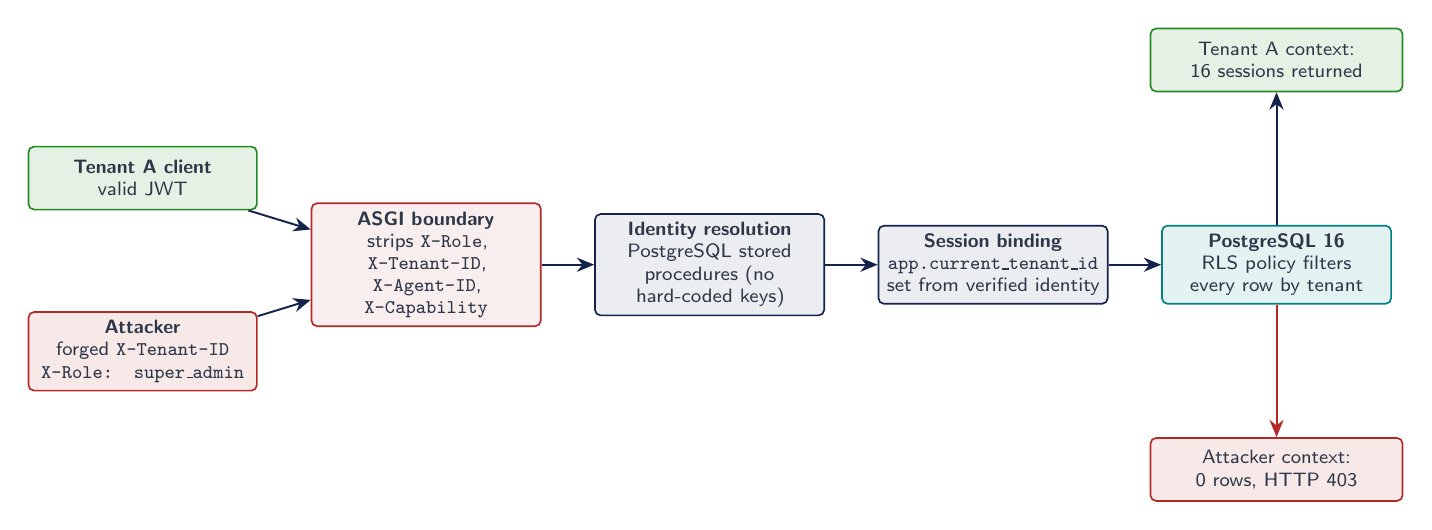
\begin{tikzpicture}
  \node[ok,minimum width=2.9cm] (ca) at (0,1.1)  {\textbf{Tenant A client}\\valid JWT};
  \node[bad,minimum width=2.9cm] (at) at (0,-1.1) {\textbf{Attacker}\\forged \texttt{X-Tenant-ID}\\\texttt{X-Role: super\_admin}};
  \node[gate,minimum width=2.9cm,text width=2.7cm] (asgi) at (3.6,0) {\textbf{ASGI boundary}\\strips \texttt{X-Role}, \texttt{X-Tenant-ID}, \texttt{X-Agent-ID}, \texttt{X-Capability}};
  \node[ctrl,minimum width=2.9cm,text width=2.7cm] (idr) at (7.2,0) {\textbf{Identity resolution}\\PostgreSQL stored procedures (no hard-coded keys)};
  \node[ctrl,minimum width=2.9cm,text width=2.7cm] (ses) at (10.8,0) {\textbf{Session binding}\\\texttt{app.current\_}\-\texttt{tenant\_id} set from verified identity};
  \node[store,minimum width=2.9cm,text width=2.7cm] (pg) at (14.4,0) {\textbf{PostgreSQL 16}\\RLS policy filters every row by tenant};
  \draw[arr] (ca) -- (asgi);
  \draw[arr] (at) -- (asgi);
  \foreach \a/\b in {asgi/idr,idr/ses,ses/pg}{\draw[arr] (\a) -- (\b);}
  \node[ok,minimum width=3.2cm] (r1) at (14.4,2.6)  {Tenant A context:\\16 sessions returned};
  \node[bad,minimum width=3.2cm] (r2) at (14.4,-2.6) {Attacker context:\\0 rows, HTTP 403};
  \draw[arr] (pg.north) -- (r1.south);
  \draw[arrr] (pg.south) -- (r2.north);
\end{tikzpicture}
\end{adjustbox}
\caption{Perimeter defence in depth: header stripping, database-resolved identity and row-level security.}
\label{fig:rls}
\end{figure}

\subsection{Dynamic information-flow control}
To keep indirect prompt injection from leaking private data, labels form a lattice \cite{denning1976}:
\begin{equation}
\text{PUBLIC}\sqsubset\text{INTERNAL}\sqsubset\text{CONFIDENTIAL}\sqsubset\text{RESTRICTED\_PII}\sqsubset\text{SECRET\_CREDENTIAL}
\end{equation}
If an agent consumes a chunk labelled $\ell_1$ and a tool return labelled $\ell_2$, its working memory inherits the least upper bound $\ell_{\text{state}}=\ell_1\sqcup\ell_2$. An agent whose state satisfies $\ell_{\text{state}}\sqsupseteq\text{CONFIDENTIAL}$ may not invoke external network tools unless declassification is explicitly approved (Figure~\ref{fig:lattice}).

\begin{figure}[!htbp]
\centering
\begin{adjustbox}{max width=\linewidth}
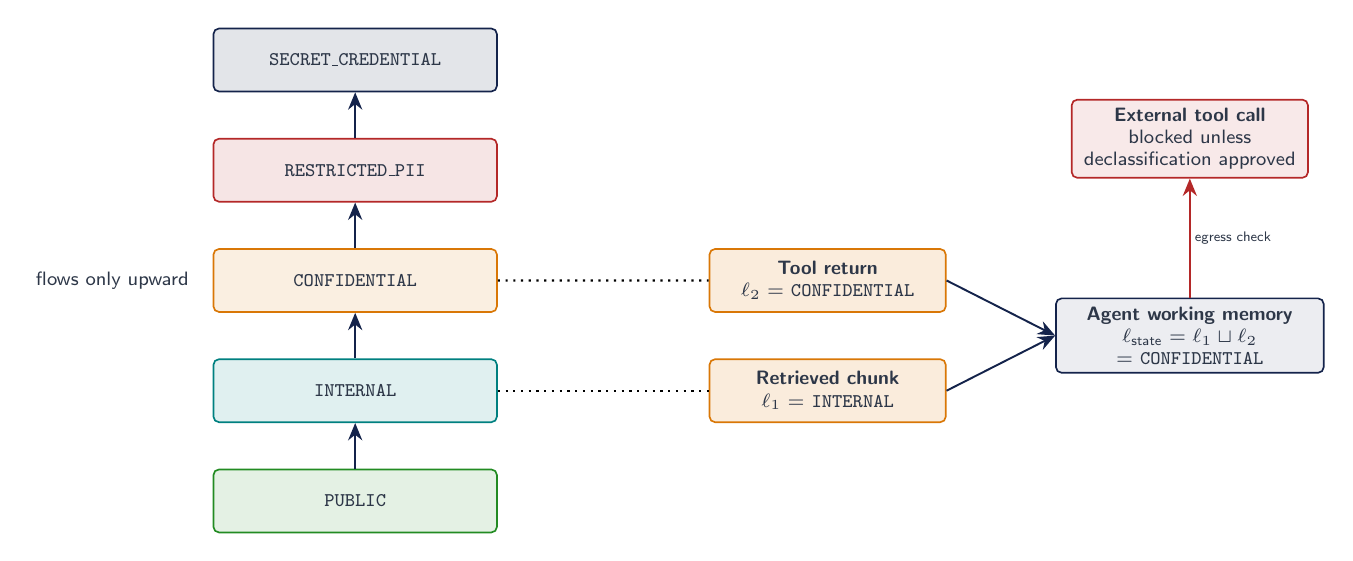
\begin{tikzpicture}
  \foreach \i/\n/\c in {0/PUBLIC/forestgreen,1/INTERNAL/accentteal,2/CONFIDENTIAL/amberorange,3/RESTRICTED\_PII/crimsonred,4/SECRET\_CREDENTIAL/primarynavy}{
    \node[box,minimum width=3.6cm,draw=\c,fill=\c!12] (L\i) at (0,{1.4*\i}) {\texttt{\n}};
  }
  \foreach \a/\b in {0/1,1/2,2/3,3/4}{\draw[arr] (L\a) -- (L\b);}
  \node[base,anchor=east] at (-2.0,2.8) {flows only upward};
  \node[warn,minimum width=3.0cm] (chunk) at (6.0,1.4) {\textbf{Retrieved chunk}\\$\ell_1=$ \texttt{INTERNAL}};
  \node[warn,minimum width=3.0cm] (tool) at (6.0,2.8)  {\textbf{Tool return}\\$\ell_2=$ \texttt{CONFIDENTIAL}};
  \draw[dotted,line width=0.8pt] (L1.east) -- (chunk.west);
  \draw[dotted,line width=0.8pt] (L2.east) -- (tool.west);
  \node[ctrl,minimum width=3.4cm] (state) at (10.6,2.1) {\textbf{Agent working memory}\\$\ell_{\text{state}}=\ell_1\sqcup\ell_2$\\$=$ \texttt{CONFIDENTIAL}};
  \draw[arr] (chunk.east) -- (state.west);
  \draw[arr] (tool.east) -- (state.west);
  \node[bad,minimum width=3.0cm] (egress) at (10.6,4.6) {\textbf{External tool call}\\blocked unless\\declassification approved};
  \draw[arrr] (state.north) -- (egress.south) node[midway,lbl,right]{egress check};
\end{tikzpicture}
\end{adjustbox}
\caption{Security lattice and taint propagation: the join of two labels governs egress.}
\label{fig:lattice}
\end{figure}

\subsection{Sliding-window blast radius}
To stop an adversary from splitting a damaging action into many benign-looking ones, Gate~3 tracks decayed cumulative risk over a window $W$:
\begin{equation}
\mathcal B(t)=\sum_{k\in\mathcal A(t,W)}\omega(a_k)\,\mathrm{Impact}(a_k)\,e^{-\lambda(t-t_k)}
\end{equation}
where $\mathcal A(t,W)$ is the set of actions in the window, $\omega(a_k)$ a per-action-class weight, $\mathrm{Impact}(a_k)$ its financial or operational sensitivity, and $\lambda>0$ a decay rate. If admitting a new action would push $\mathcal B(t)$ above $\mathcal B_{\max}$, it is denied regardless of its individual risk (Figure~\ref{fig:blast}; this gate is a specification).

\begin{figure}[!htbp]
\centering
\begin{adjustbox}{max width=\linewidth}
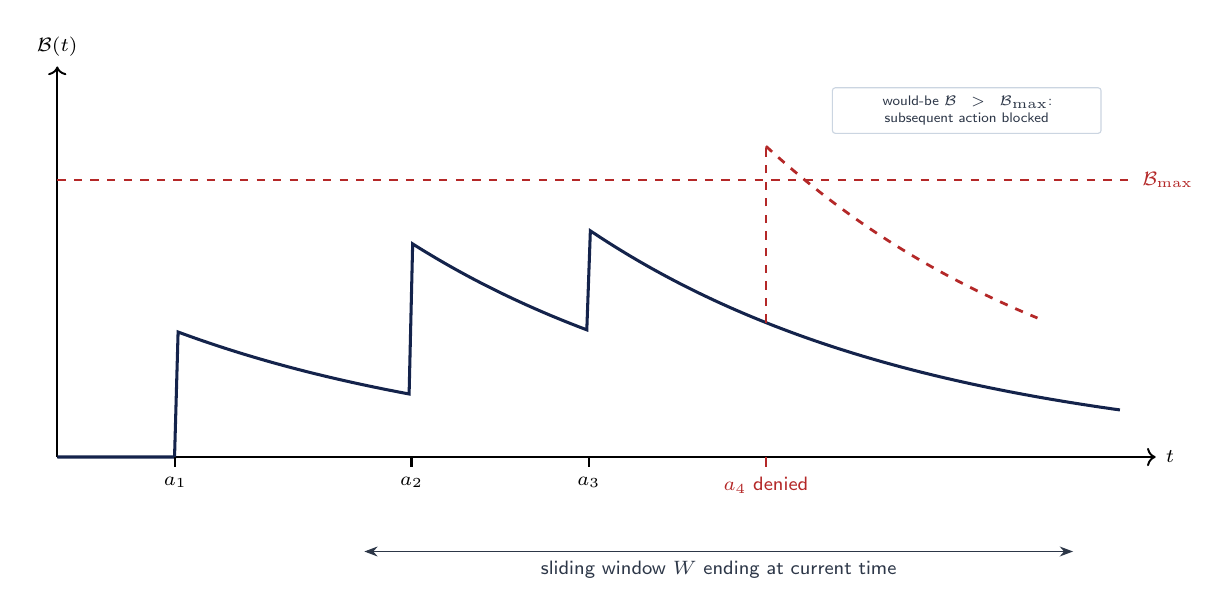
\begin{tikzpicture}[x=1.5cm,y=1.6cm]
  \draw[->,line width=0.7pt] (0,0) -- (9.3,0) node[right,font=\sffamily\scriptsize]{$t$};
  \draw[->,line width=0.7pt] (0,0) -- (0,3.1) node[above,font=\sffamily\scriptsize]{$\mathcal B(t)$};
  \draw[crimsonred,dashed,line width=0.8pt] (0,2.2) -- (9.1,2.2) node[right,font=\sffamily\scriptsize,text=crimsonred]{$\mathcal B_{\max}$};
  % executed actions: curve with a1..a3
  \draw[primarynavy,line width=1.1pt,domain=0:9,samples=300]
    plot (\x,{ifthenelse(\x>1,1.0*exp(-0.35*(\x-1)),0)+ifthenelse(\x>3,1.2*exp(-0.35*(\x-3)),0)+ifthenelse(\x>4.5,0.8*exp(-0.35*(\x-4.5)),0)});
  % would-be curve if a4 were admitted
  \draw[crimsonred,dashed,line width=1.0pt,domain=6.0:8.3,samples=100]
    plot (\x,{1.0*exp(-0.35*(\x-1))+1.2*exp(-0.35*(\x-3))+0.8*exp(-0.35*(\x-4.5))+1.4*exp(-0.35*(\x-6))});
  \draw[crimsonred,dashed,line width=1.0pt] (6,1.066) -- (6,2.466);
  \foreach \t/\n in {1/1,3/2,4.5/3}{\draw[line width=0.8pt] (\t,0) -- (\t,-0.08); \node[below,font=\sffamily\scriptsize] at (\t,-0.08) {$a_{\n}$};}
  \draw[crimsonred,line width=0.8pt] (6,0) -- (6,-0.08);
  \node[below,font=\sffamily\scriptsize,text=crimsonred,align=center] at (6,-0.08) {$a_4$ denied};
  \node[note,text width=3.2cm,fill=white] at (7.7,2.75) {would-be $\mathcal B>\mathcal B_{\max}$:\\subsequent action blocked};
  \draw[{Stealth}-{Stealth},darkslate] (2.6,-0.75) -- (8.6,-0.75) node[midway,below,font=\sffamily\scriptsize]{sliding window $W$ ending at current time};
\end{tikzpicture}
\end{adjustbox}
\caption{Illustrative blast-radius dynamics ($\lambda=0.35$, $\omega=1$, impacts 1.0, 1.2, 0.8, 1.4): the fourth action would breach $\mathcal B_{\max}$ and is denied.}
\label{fig:blast}
\end{figure}

\subsection{Tamper-evident audit ledger}
Every decision, action and policy evaluation is chained:
\begin{equation}
H_t=\mathrm{SHA\text{-}256}\big(H_{t-1}\,\Vert\,\text{TransactionID}\,\Vert\,\text{Timestamp}\,\Vert\,\text{ActionPayload}\,\Vert\,\text{Decision}\big)
\end{equation}
Changing any historical record invalidates the hashes of all later records, supporting forensic non-repudiation for SOC~2, HIPAA and EU AI Act audits (Figure~\ref{fig:hashchain}).

\begin{figure}[!htbp]
\centering
\begin{adjustbox}{max width=\linewidth}
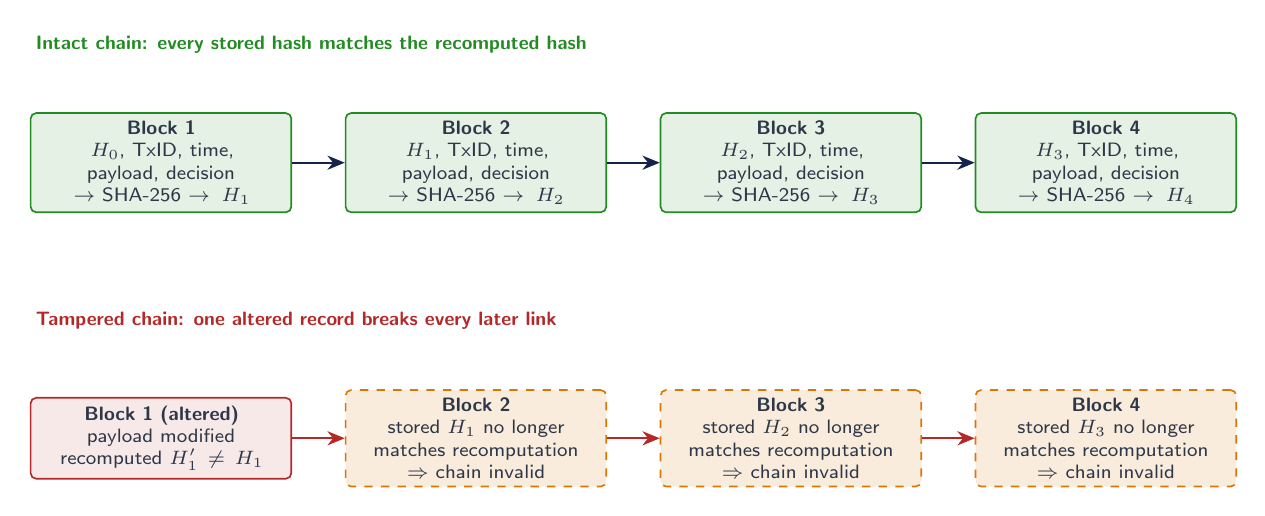
\begin{tikzpicture}
  \node[base,font=\sffamily\scriptsize\bfseries,text=forestgreen,anchor=west] at (-1.7,1.5) {Intact chain: every stored hash matches the recomputed hash};
  \foreach \i in {0,1,2,3}{
    \pgfmathtruncatemacro{\k}{\i+1}
    \node[ok,minimum width=3.3cm,text width=3.1cm] (a\i) at (\i*4.0,0) {\textbf{Block \k}\\$H_{\i}$, TxID, time,\\payload, decision\\$\rightarrow$ SHA-256 $\rightarrow H_{\k}$};
  }
  \foreach \a/\b in {0/1,1/2,2/3}{\draw[arr] (a\a) -- (a\b);}
  \node[base,font=\sffamily\scriptsize\bfseries,text=crimsonred,anchor=west] at (-1.7,-2.0) {Tampered chain: one altered record breaks every later link};
  \node[bad,minimum width=3.3cm,text width=3.1cm] (t0) at (0,-3.5) {\textbf{Block 1 (altered)}\\payload modified\\recomputed $H_1'\neq H_1$};
  \foreach \i in {1,2,3}{
    \pgfmathtruncatemacro{\k}{\i+1}
    \node[warn,minimum width=3.3cm,text width=3.1cm,dashed] (t\i) at (\i*4.0,-3.5) {\textbf{Block \k}\\stored $H_{\i}$ no longer\\matches recomputation\\$\Rightarrow$ chain invalid};
  }
  \foreach \a/\b in {0/1,1/2,2/3}{\draw[arrr] (t\a) -- (t\b);}
\end{tikzpicture}
\end{adjustbox}
\caption{SHA-256 hash-chained audit ledger: intact versus tampered chain.}
\label{fig:hashchain}
\end{figure}

%==============================================================================
\section{Gate 4: Output Assurance and the Verification Engine}\label{sec:gate4}
%==============================================================================

\subsection{Evidence signals}
The MIRAGE 2.x scientific pipeline is the algorithmic core of Gate~4. Compound text is split into atomic claims, each verified through orthogonal signals (Table~\ref{tab:signals_matrix}, Figure~\ref{fig:engine}).

\begin{table}[!htbp]
\centering\small
\renewcommand{\arraystretch}{1.2}
\rowcolors{2}{white}{lightgreybg}
\begin{tabularx}{\linewidth}{@{}L{3.2cm} L{3.6cm} L{2.4cm} Y@{}}
\hdrrow \hc{Signal} & \hc{Technology} & \hc{Measured latency} & \hc{Failure mitigated}\\
\toprule
\textbf{RAV} -- dense retrieval & Qdrant HNSW + MPNet-768 \cite{song2020} & $\sim$45\,ms & Fabrications unsupported by the reference corpus.\\
\textbf{SCS} -- consistency sampling & Parallel Groq sampling, $T=0.7$ & $\sim$800\,ms ($<$2\,ms on cache hit) & Semantic dispersion under model uncertainty.\\
\textbf{NLI} -- entailment & DeBERTa-v3 cross-encoder \cite{he2021v3} & $\sim$80\,ms & Contradiction against verified references.\\
\textbf{VGS} -- visual grounding & OpenCLIP + LLaVA-1.6 & $\sim$30\,ms / $\sim$900\,ms & Fabricated visual objects.\\
\textbf{ICS} -- internal consistency & Semantic chunk consistency & $\sim$25\,ms & Self-contradiction across paragraphs.\\
\bottomrule
\end{tabularx}
\caption{Multi-signal evidence matrix of the Gate 4 verification engine.}
\label{tab:signals_matrix}
\end{table}

\begin{figure}[!htbp]
\centering
\begin{adjustbox}{max width=\linewidth}
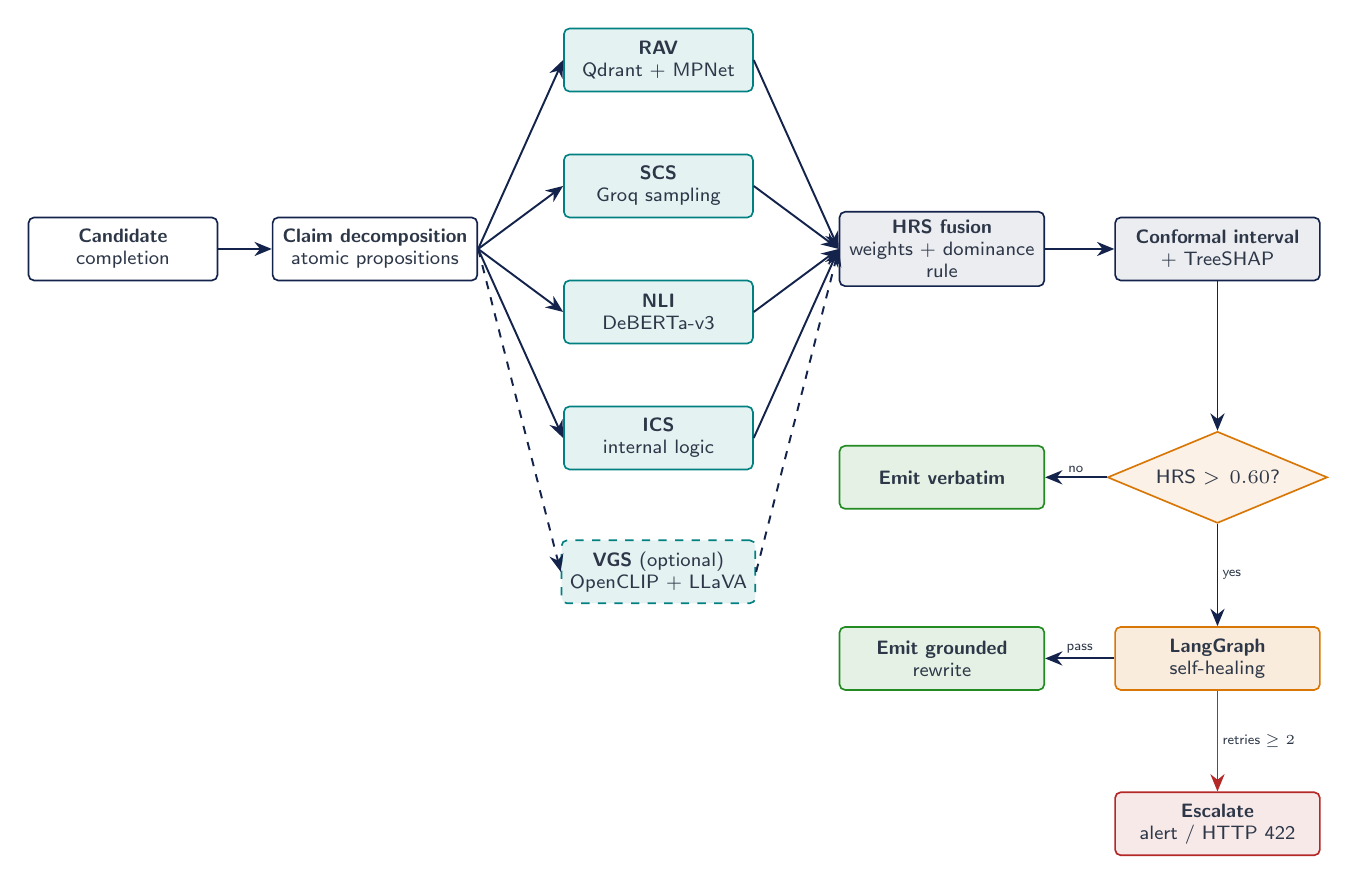
\begin{tikzpicture}
  \node[box,minimum width=2.4cm] (cand) at (0,0)   {\textbf{Candidate}\\completion};
  \node[box,minimum width=2.6cm] (dec) at (3.2,0)  {\textbf{Claim decomposition}\\atomic propositions};
  \foreach \i/\n/\s in {0/RAV/{Qdrant + MPNet},1/SCS/{Groq sampling},2/NLI/{DeBERTa-v3},3/ICS/{internal logic}}{
    \node[store,minimum width=2.4cm] (sg\i) at (6.8,{2.4-1.6*\i}) {\textbf{\n}\\\s};
    \draw[arr] (dec.east) -- (sg\i.west);
  }
  \node[store,minimum width=2.4cm,dashed] (vgs) at (6.8,-4.1) {\textbf{VGS} (optional)\\OpenCLIP + LLaVA};
  \draw[arrd] (dec.east) -- (vgs.west);
  \node[ctrl,minimum width=2.6cm] (fus) at (10.4,0) {\textbf{HRS fusion}\\weights + dominance\\rule};
  \foreach \i in {0,1,2,3}{\draw[arr] (sg\i.east) -- (fus.west);}
  \draw[arrd] (vgs.east) -- (fus.west);
  \node[ctrl,minimum width=2.6cm] (conf) at (13.9,0) {\textbf{Conformal interval}\\+ TreeSHAP};
  \draw[arr] (cand) -- (dec);
  \draw[arr] (fus) -- (conf);
  \node[dec,text width=2.1cm] (dg) at (13.9,-2.9) {HRS $>0.60$?};
  \draw[arr] (conf) -- (dg);
  \node[ok,minimum width=2.6cm] (emit) at (10.4,-2.9) {\textbf{Emit verbatim}};
  \node[warn,minimum width=2.6cm] (heal) at (13.9,-5.2) {\textbf{LangGraph}\\self-healing};
  \node[ok,minimum width=2.6cm] (emit2) at (10.4,-5.2) {\textbf{Emit grounded}\\rewrite};
  \node[bad,minimum width=2.6cm] (esc) at (13.9,-7.3) {\textbf{Escalate}\\alert / HTTP 422};
  \draw[arr] (dg.west) -- (emit.east) node[midway,lbl,above]{no};
  \draw[arr] (dg.south) -- (heal.north) node[midway,lbl,right]{yes};
  \draw[arr] (heal.west) -- (emit2.east) node[midway,lbl,above]{pass};
  \draw[arrr] (heal.south) -- (esc.north) node[midway,lbl,right]{retries $\ge2$};
\end{tikzpicture}
\end{adjustbox}
\caption{Gate~4 verification engine: from claim decomposition to emission, self-healing or escalation.}
\label{fig:engine}
\end{figure}

\subsection{HRS fusion and the dominance rule}
Each signal is normalised so that higher means riskier. The claim-level Hallucination Risk Score is
\begin{equation}
\mathrm{HRS}(c_i)=w_1\,\mathrm{RAV}(c_i)+w_2\,\mathrm{SCS}(c_i)+w_3\,\mathrm{NLI}(c_i)+w_4\,\mathrm{ICS}(c_i),
\end{equation}
with canonical weights $w_1=0.35$, $w_2=0.30$, $w_3=0.25$, $w_4=0.10$ (summing to one). Because a response containing one fatal falsehood is not safe merely because the rest is accurate, the \textbf{critical-hallucination dominance rule} is applied, where $w_{\text{crit}}(c_i)$ is the criticality weight of claim $c_i$:
\begin{equation}
\mathrm{HRS}_{\text{resp}}=\max\!\left(\frac{\sum_{i=1}^{K}w_{\text{crit}}(c_i)\,\mathrm{HRS}(c_i)}{\sum_{i=1}^{K}w_{\text{crit}}(c_i)},\ 0.80\cdot\max_{1\le i\le K}\mathrm{HRS}(c_i)\right)
\end{equation}

\subsection{Split-conformal calibration and attribution}
Prediction intervals are calibrated on held-out non-conformity scores $\{s_i\}_{i=1}^n$ \cite{vovk2005,lei2018,angelopoulos2021}:
\begin{equation}
\hat q=\mathrm{Quantile}\!\left(\{s_i\}_{i=1}^{n},\ \frac{\lceil (n+1)(1-\alpha)\rceil}{n}\right),\qquad
\mathcal C(\mathbf x)=\big[\max(0,\mathrm{HRS}-\hat q),\ \min(1,\mathrm{HRS}+\hat q)\big]
\end{equation}
At $1-\alpha=0.95$ and $n=1{,}000$ calibration examples, the measured $\hat q=0.0650$ gives an interval width of $0.130<0.20$. The coverage guarantee is \emph{marginal} and assumes calibration and deployment data are exchangeable; the Mondrian variant provides coverage per category. TreeSHAP decomposes the score additively, $\mathrm{HRS}(\mathbf x)=\phi_0+\sum_{j=1}^{M}\phi_j(\mathbf x)$ \cite{lundberg2017,lundberg2020}.

\subsection{LangGraph closed-loop self-healing}
When $\mathrm{HRS}>0.60$, a compiled LangGraph state machine isolates contradicted claims, retrieves targeted Qdrant evidence, performs a grounded rewrite and applies a mandatory re-verification gate $\mathrm{HRS}_{\text{rewrite}}\le0.30$ before emission (Figure~\ref{fig:langgraph}).

\begin{figure}[!htbp]
\centering
\begin{adjustbox}{max width=\linewidth}
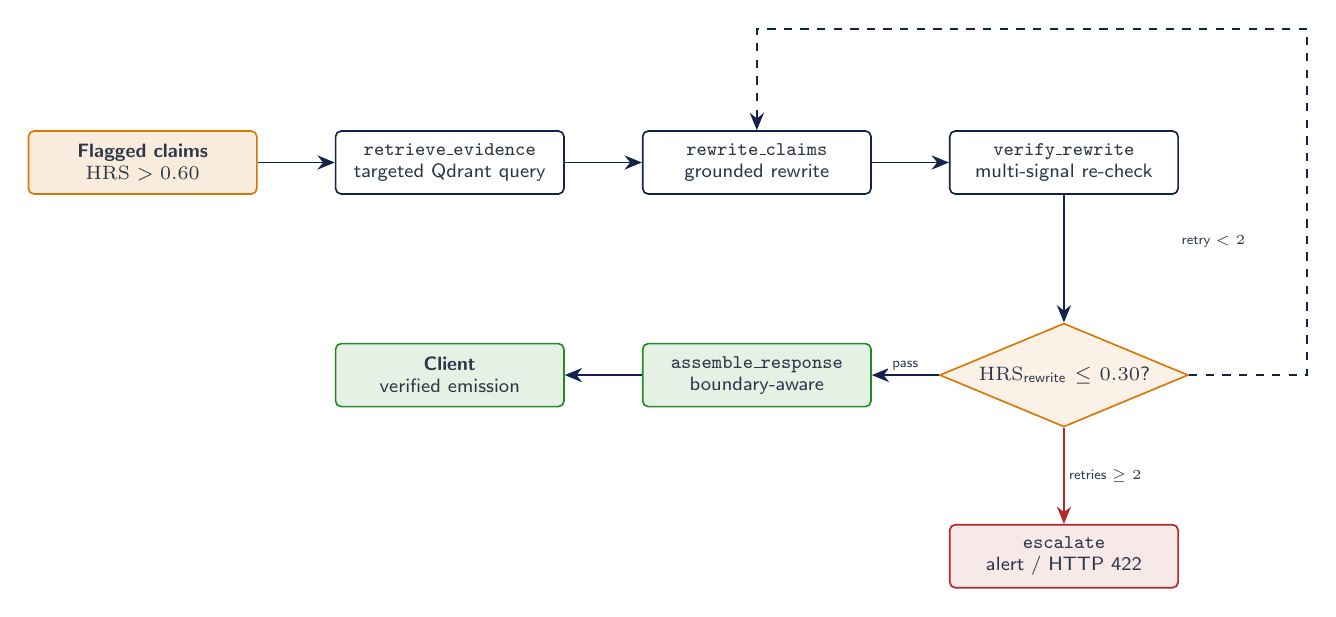
\begin{tikzpicture}
  \node[warn,minimum width=2.9cm] (flag) at (0,0)    {\textbf{Flagged claims}\\$\mathrm{HRS}>0.60$};
  \node[box,minimum width=2.9cm] (ret) at (3.9,0)    {\textbf{\texttt{retrieve\_evidence}}\\targeted Qdrant query};
  \node[box,minimum width=2.9cm] (rew) at (7.8,0)    {\textbf{\texttt{rewrite\_claims}}\\grounded rewrite};
  \node[box,minimum width=2.9cm] (ver) at (11.7,0)   {\textbf{\texttt{verify\_rewrite}}\\multi-signal re-check};
  \node[dec,text width=2.4cm] (gt) at (11.7,-2.7)    {$\mathrm{HRS}_{\text{rewrite}}\le0.30$?};
  \node[ok,minimum width=2.9cm] (asm) at (7.8,-2.7)  {\textbf{\texttt{assemble\_response}}\\boundary-aware};
  \node[ok,minimum width=2.9cm] (cli) at (3.9,-2.7)  {\textbf{Client}\\verified emission};
  \node[bad,minimum width=2.9cm] (esc) at (11.7,-5.0) {\textbf{\texttt{escalate}}\\alert / HTTP 422};
  \foreach \a/\b in {flag/ret,ret/rew,rew/ver,ver/gt}{\draw[arr] (\a) -- (\b);}
  \draw[arr] (gt.west) -- (asm.east) node[midway,lbl,above]{pass};
  \draw[arr] (asm) -- (cli);
  \draw[arrr] (gt.south) -- (esc.north) node[midway,lbl,right]{retries $\ge2$};
  \draw[arrd] (gt.east) -- ++(1.5,0) |- (7.8,1.7) -- (rew.north);
  \node[lbl] at (13.6,-1.0) {retry $<2$};
\end{tikzpicture}
\end{adjustbox}
\caption{LangGraph closed-loop self-correction with a mandatory re-verification gate.}
\label{fig:langgraph}
\end{figure}

%==============================================================================
\section{Validated Empirical Telemetry}
%==============================================================================

\subsection{Runtime model identity probes}
Direct probes of the Groq inference endpoint (\texttt{api.groq.com/openai/v1/chat/completions}) established production telemetry:
\begin{itemize}[leftmargin=*,itemsep=1pt]
  \item \textbf{Active production model:} \texttt{allam-2-7b} (system fingerprint \texttt{fp\_ff744b2c7a}).
  \item \textbf{Measured latency:} generation 15.18\,ms, queue time 46.18\,ms.
  \item \textbf{Upstream deprecation:} \texttt{llama-3.1-70b-versatile} and \texttt{llama-3.1-8b-instant} were decommissioned (HTTP~400); all harnesses were aligned to \texttt{allam-2-7b}.
\end{itemize}

\subsection{Grounded versus hallucinated verification}
\begin{table}[!htbp]
\centering\small
\renewcommand{\arraystretch}{1.2}
\rowcolors{2}{white}{lightgreybg}
\begin{tabularx}{\linewidth}{@{}L{3.1cm} Y Y@{}}
\hdrrow \hc{Metric} & \hc{Scenario A: grounded} & \hc{Scenario B: contradicted}\\
\toprule
Prompt & ``Who discovered penicillin and when?'' & ``Who discovered penicillin and where?''\\
Candidate & ``Alexander Fleming discovered penicillin in 1928 at St.\ Mary's Hospital in London.'' & ``Alexander Fleming discovered penicillin in 1999 at Harvard University in Boston.''\\
Qdrant match & Chunk \texttt{doc\_a745\dots}, similarity 0.8164 & Chunk \texttt{doc\_a745\dots}, similarity 0.7912\\
Claims & $c_1$ Fleming 1928: \texttt{SUPPORTED} (0.190); $c_2$ St.\ Mary's: \texttt{NEUTRAL} (0.446) & $c_1$ Fleming 1999 Harvard: \texttt{CONTRADICTED} (0.850)\\
Overall HRS & \textbf{0.2863} (low/medium) & \textbf{0.8500} (critical)\\
Conformal interval & [0.2213, 0.3513] & [0.7650, 0.9350]\\
Attribution (TreeSHAP, as reported) & SCS 0.570, RAV 0.266, NLI 0.123 & NLI 0.520, SCS 0.320, RAV 0.160\\
LangGraph & Bypassed ($\le0.60$) & Triggered ($>0.60$)\\
Rewritten output & Original preserved verbatim & ``Alexander Fleming discovered penicillin in 1928 at St.\ Mary's Hospital in London.''\\
Re-verification & N/A & $\mathrm{HRS}_{\text{rewrite}}=\mathbf{0.0440}$ (gate $\le0.30$ passed)\\
Emitted status & Direct emission & Grounded rewrite emitted\\
\bottomrule
\end{tabularx}
\caption{Live telemetry captured on two production scenarios.}
\label{tab:telemetry_table}
\end{table}

\begin{figure}[!htbp]
\centering
\begin{adjustbox}{max width=\linewidth}
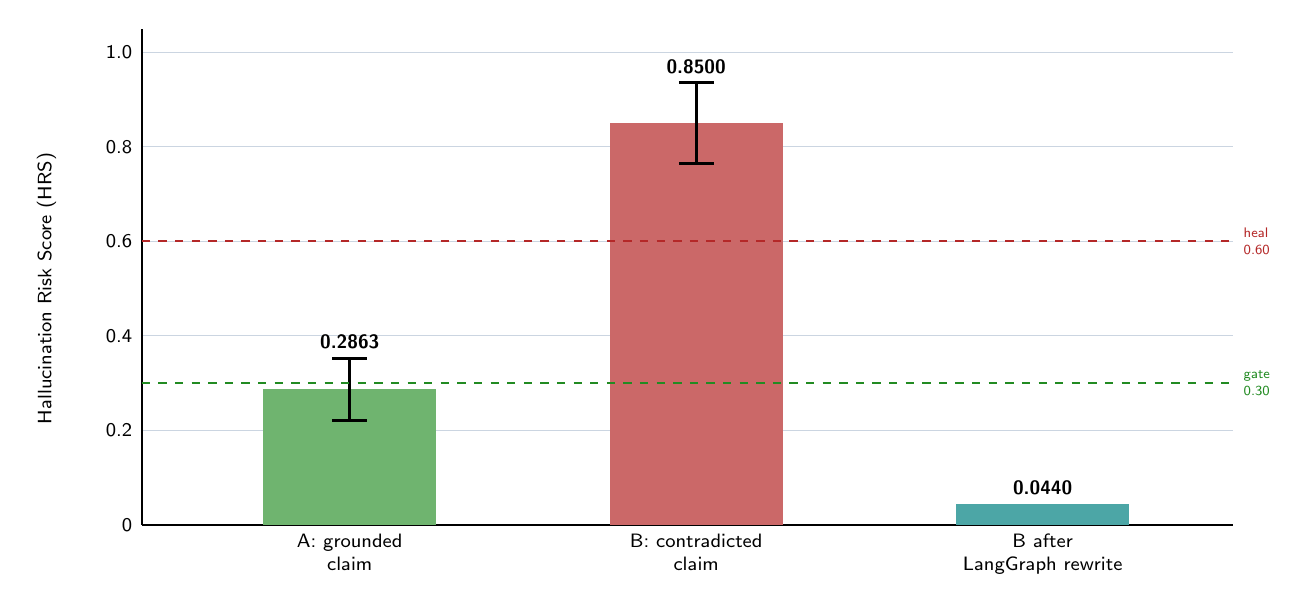
\begin{tikzpicture}[x=2.2cm,y=6cm]
  \foreach \v in {0,0.2,0.4,0.6,0.8,1.0}{
    \draw[bordergrey,line width=0.4pt] (0,\v) -- (6.3,\v);
    \node[left,font=\sffamily\scriptsize] at (0,\v) {\v};
  }
  \draw[line width=0.7pt] (0,0) -- (6.3,0);
  \draw[line width=0.7pt] (0,0) -- (0,1.05);
  \node[rotate=90,font=\sffamily\scriptsize] at (-0.55,0.5) {Hallucination Risk Score (HRS)};
  % bars
  \fill[forestgreen!65] (0.7,0) rectangle (1.7,0.2863);
  \fill[crimsonred!70]  (2.7,0) rectangle (3.7,0.85);
  \fill[accentteal!70]  (4.7,0) rectangle (5.7,0.044);
  % conformal intervals
  \draw[line width=1.1pt] (1.2,0.2213) -- (1.2,0.3513); \draw[line width=1.1pt] (1.1,0.2213) -- (1.3,0.2213); \draw[line width=1.1pt] (1.1,0.3513) -- (1.3,0.3513);
  \draw[line width=1.1pt] (3.2,0.765) -- (3.2,0.935);   \draw[line width=1.1pt] (3.1,0.765) -- (3.3,0.765);   \draw[line width=1.1pt] (3.1,0.935) -- (3.3,0.935);
  % values
  \node[above,font=\sffamily\scriptsize\bfseries] at (1.2,0.3513) {0.2863};
  \node[above,font=\sffamily\scriptsize\bfseries] at (3.2,0.935) {0.8500};
  \node[above,font=\sffamily\scriptsize\bfseries] at (5.2,0.044) {0.0440};
  % thresholds
  \draw[crimsonred,dashed,line width=0.9pt] (0,0.6) -- (6.3,0.6) node[right,font=\sffamily\tiny,text=crimsonred,align=left]{heal\\0.60};
  \draw[forestgreen,dashed,line width=0.9pt] (0,0.3) -- (6.3,0.3) node[right,font=\sffamily\tiny,text=forestgreen,align=left]{gate\\0.30};
  % category labels
  \node[font=\sffamily\scriptsize,align=center,below] at (1.2,0) {A: grounded\\claim};
  \node[font=\sffamily\scriptsize,align=center,below] at (3.2,0) {B: contradicted\\claim};
  \node[font=\sffamily\scriptsize,align=center,below] at (5.2,0) {B after\\LangGraph rewrite};
\end{tikzpicture}
\end{adjustbox}
\caption{HRS for the two live scenarios with 95\% conformal intervals ($\hat q=0.0650$). The rewrite drops scenario B from 0.85 to 0.044, below the 0.30 re-verification gate.}
\label{fig:telemetry}
\end{figure}

\subsection{Persistence and fault-injection probes}
\begin{itemize}[leftmargin=*,itemsep=1pt]
  \item \textbf{Row-level security probe.} With \texttt{app.current\_tenant\_id} set to \texttt{'tenant\_attacker'}, queries returned 0 rows; the authorised tenant context returned all 16 sessions; cross-tenant access returned HTTP~403.
  \item \textbf{Circuit-breaker fault injection.} Port failures injected into Qdrant tripped PyBreaker to \texttt{OPEN} within three failures; the fallback sparsity penalty applied without any unhandled HTTP~500.
\end{itemize}

%==============================================================================
\section{Cost Optimisation: The Verification Escalation Ladder}
%==============================================================================
Assurance must not multiply cost and latency. MIRAGE handles each case at the cheapest rung that can resolve it (Figure~\ref{fig:ladder}); expensive rungs run only when cheaper ones are inconclusive or policy requires them.

\begin{figure}[!htbp]
\centering
\begin{adjustbox}{max width=\linewidth}
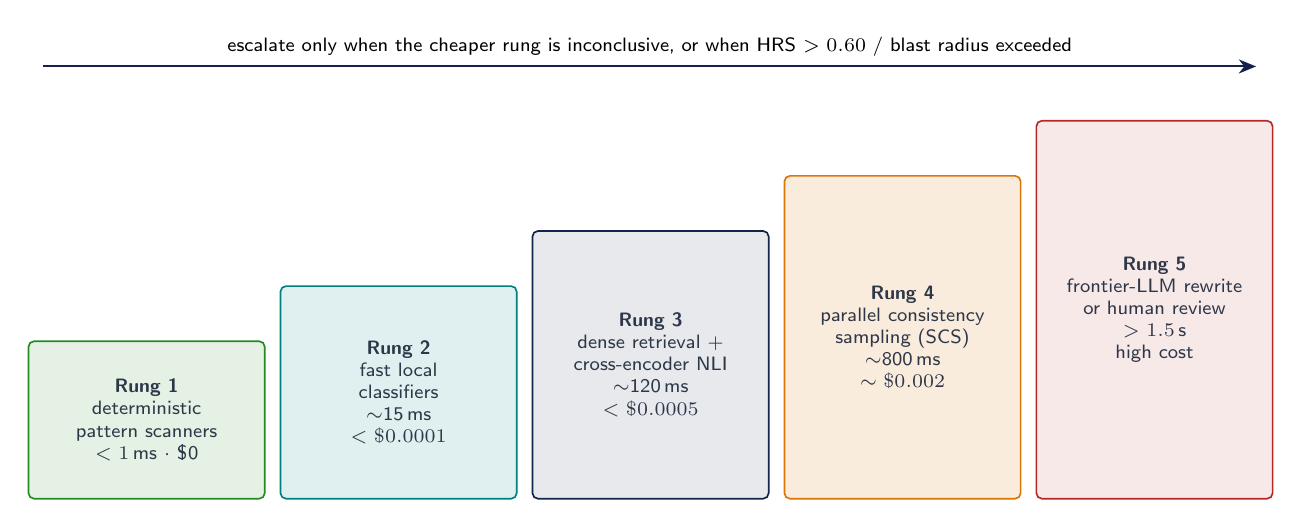
\begin{tikzpicture}
  \node[box,anchor=south west,minimum width=3.0cm,minimum height=2.0cm,draw=forestgreen,fill=forestgreen!12]   at (0,0)    {\textbf{Rung 1}\\deterministic\\pattern scanners\\$<1$\,ms $\cdot$ \$0};
  \node[box,anchor=south west,minimum width=3.0cm,minimum height=2.7cm,draw=accentteal,fill=accentteal!12]       at (3.2,0)  {\textbf{Rung 2}\\fast local\\classifiers\\$\sim$15\,ms\\$<\$0.0001$};
  \node[box,anchor=south west,minimum width=3.0cm,minimum height=3.4cm,draw=primarynavy,fill=primarynavy!10]    at (6.4,0)  {\textbf{Rung 3}\\dense retrieval +\\cross-encoder NLI\\$\sim$120\,ms\\$<\$0.0005$};
  \node[box,anchor=south west,minimum width=3.0cm,minimum height=4.1cm,draw=amberorange,fill=amberorange!14]    at (9.6,0)  {\textbf{Rung 4}\\parallel consistency\\sampling (SCS)\\$\sim$800\,ms\\$\sim\$0.002$};
  \node[box,anchor=south west,minimum width=3.0cm,minimum height=4.8cm,draw=crimsonred,fill=crimsonred!10]      at (12.8,0) {\textbf{Rung 5}\\frontier-LLM rewrite\\or human review\\$>1.5$\,s\\high cost};
  \draw[arr] (0.2,5.5) -- (15.6,5.5) node[midway,above,font=\sffamily\scriptsize]{escalate only when the cheaper rung is inconclusive, or when HRS $>0.60$ / blast radius exceeded};
\end{tikzpicture}
\end{adjustbox}
\caption{Verification escalation ladder: cost and latency grow with each rung.}
\label{fig:ladder}
\end{figure}

%==============================================================================
\section{Comprehensive Competitive Landscape}
%==============================================================================
MIRAGE 3.0 is compared with nine commercial and academic systems. The table is split into two parts so every column stays legible; cell entries reflect each tool's public documentation at the time of writing and should be re-verified before external publication.

\begin{table}[!htbp]
\centering\scriptsize
\renewcommand{\arraystretch}{1.25}
\rowcolors{2}{white}{lightgreybg}
\begin{tabularx}{\linewidth}{@{}L{2.2cm} Y Y Y Y Y@{}}
\hdrrow \hc{Dimension} & \hc{MIRAGE 3.0} & \hc{SelfCheckGPT} & \hc{FActScore} & \hc{Guardrails AI} & \hc{NeMo Guardrails}\\
\toprule
Category & Execution fabric & Offline algorithm & Offline evaluation & Python SDK & Dialog framework (Colang)\\
Assurance scope & \textbf{Five gates} & Output only & Output only & Input / output & Input / output\\
Action governance & \textbf{Capability ABAC} & None & None & None & Programmable\\
Reality verification & \textbf{Seven-state probes} & None & None & None & None\\
Dynamic IFC & \textbf{Taint tracking} & None & None & None & None\\
Multi-signal & \textbf{4+1 orthogonal} & SCS only & RAG + NLI & Regex / LLM validators & Vector embeddings\\
Uncertainty & \textbf{Split-conformal} & None & None & None & None\\
Self-correction & \textbf{LangGraph gate} & None & None & Exception handling & Flow redirect\\
Multi-tenancy & \textbf{Postgres RLS} & None & None & In-memory & None\\
Audit ledger & \textbf{SHA-256 chain} & None & None & Plain logs & Plain logs\\
Deployment & \textbf{Sovereign VPC} & Script & Script & Microservice & Container\\
\bottomrule
\end{tabularx}
\caption{Architectural comparison, part A: academic baselines and guardrail libraries.}
\label{tab:competitors_a}
\end{table}

\begin{table}[!htbp]
\centering\scriptsize
\renewcommand{\arraystretch}{1.25}
\rowcolors{2}{white}{lightgreybg}
\begin{tabularx}{\linewidth}{@{}L{2.1cm} Y Y Y Y Y Y@{}}
\hdrrow \hc{Dimension} & \hc{MIRAGE 3.0} & \hc{Cleanlab TLM} & \hc{Galileo} & \hc{TruLens} & \hc{Langfuse} & \hc{Bedrock Guardrails}\\
\toprule
Category & Execution fabric & Scoring API & SaaS platform & SDK evaluation & Tracing SaaS & Cloud proxy\\
Assurance scope & \textbf{Five gates} & Output only & Output only & Output only & Observability & Input / output filters\\
Action governance & \textbf{Capability ABAC} & None & None & None & None & None\\
Reality verification & \textbf{Seven-state probes} & None & None & None & None & None\\
Dynamic IFC & \textbf{Taint tracking} & None & None & None & None & None\\
Multi-signal & \textbf{4+1 orthogonal} & Perplexity-based & LLM-as-judge & RAG triad & Metadata & Regex / keywords\\
Uncertainty & \textbf{Split-conformal} & Heuristic & Heuristic & None & None & None\\
Self-correction & \textbf{LangGraph gate} & Best-of-N & None & None & None & Drop / mask\\
Multi-tenancy & \textbf{Postgres RLS} & Cloud tenant & SaaS tenant & SaaS tenant & SaaS tenant & AWS IAM\\
Audit ledger & \textbf{SHA-256 chain} & Plain logs & Plain logs & OpenTelemetry & ClickHouse & CloudWatch\\
Deployment & \textbf{Sovereign VPC} & Proprietary & Proprietary & Open / cloud & Open / cloud & AWS only\\
\bottomrule
\end{tabularx}
\caption{Architectural comparison, part B: commercial evaluation and cloud platforms.}
\label{tab:competitors_b}
\end{table}

Figure~\ref{fig:coverage} visualises the lifecycle coverage implied by the ``assurance scope'' and ``action governance'' rows.

\begin{figure}[!htbp]
\centering
\begin{adjustbox}{max width=\linewidth}
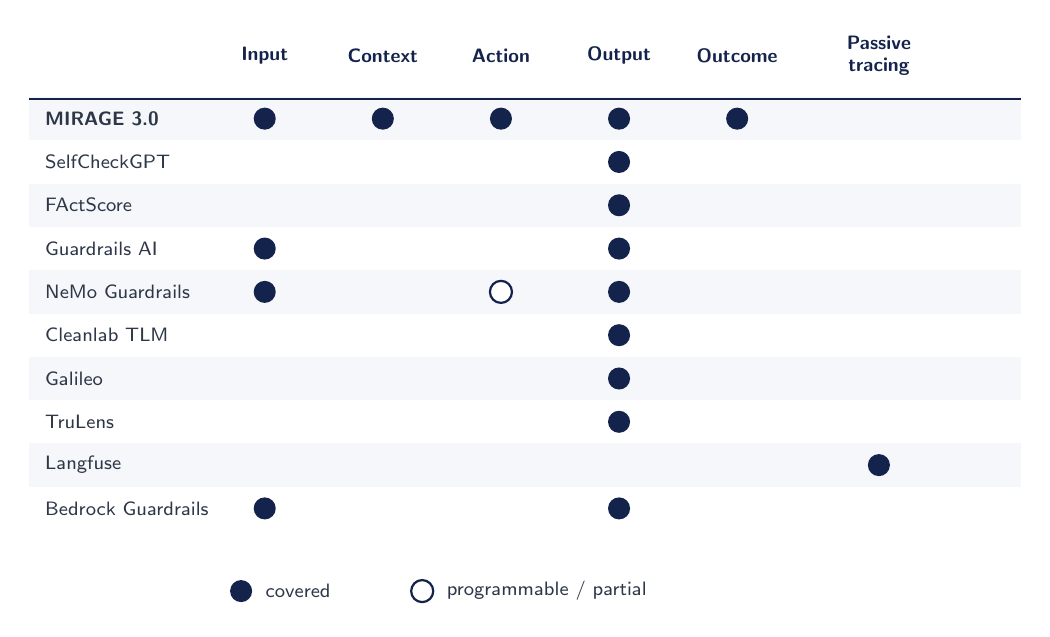
\begin{tikzpicture}
  \foreach \i in {0,2,4,6,8}{\fill[lightgreybg] (-3.0,{-0.55*\i-0.275}) rectangle (9.6,{-0.55*\i+0.275});}
  \foreach \x/\t in {0/{Input},1.5/{Context},3/{Action},4.5/{Output},6/{Outcome},7.8/{Passive\\tracing}}{
    \node[base,font=\sffamily\scriptsize\bfseries,text=primarynavy] at (\x,0.8) {\t};
  }
  \draw[primarynavy,line width=0.6pt] (-3.0,0.25) -- (9.6,0.25);
  \foreach \i/\t in {0/{\textbf{MIRAGE 3.0}},1/SelfCheckGPT,2/FActScore,3/{Guardrails AI},4/{NeMo Guardrails},5/{Cleanlab TLM},6/{Galileo},7/{TruLens},8/{Langfuse},9/{Bedrock Guardrails}}{
    \node[base,anchor=west,align=left] at (-2.9,{-0.55*\i}) {\t};
  }
  % MIRAGE
  \dotp{0}{0} \dotp{1.5}{0} \dotp{3}{0} \dotp{4.5}{0} \dotp{6}{0}
  % output-only tools
  \dotp{4.5}{-0.55} \dotp{4.5}{-1.1}
  % guardrails ai
  \dotp{0}{-1.65} \dotp{4.5}{-1.65}
  % nemo
  \dotp{0}{-2.2} \dotr{3}{-2.2} \dotp{4.5}{-2.2}
  % cleanlab, galileo, trulens
  \dotp{4.5}{-2.75} \dotp{4.5}{-3.3} \dotp{4.5}{-3.85}
  % langfuse
  \dotp{7.8}{-4.4}
  % bedrock
  \dotp{0}{-4.95} \dotp{4.5}{-4.95}
  \dotp{-0.3}{-6.0} \node[base,anchor=west] at (-0.1,-6.0) {covered};
  \dotr{2.0}{-6.0}  \node[base,anchor=west] at (2.2,-6.0) {programmable / partial};
\end{tikzpicture}
\end{adjustbox}
\caption{Lifecycle coverage of compared systems, derived from the ``assurance scope'' and ``action governance'' rows.}
\label{fig:coverage}
\end{figure}

\subsection{Architectural differentiation}
\begin{itemize}[leftmargin=*,itemsep=2pt]
  \item \textbf{Versus guardrail libraries (Guardrails AI, NeMo).} They rely on procedural validators or dialog flows; neither provides calibrated probabilistic risk scores or database-enforced multi-tenancy.
  \item \textbf{Versus observability platforms (Langfuse, TruLens).} They record traces after the fact; they cannot block an unauthorised action inline, enforce capabilities or verify outcomes.
  \item \textbf{Versus offline evaluators (SelfCheckGPT \cite{manakul2023}, FActScore \cite{min2023}).} These are research algorithms, not sub-second inline mediators, and offer no self-correction loop.
\end{itemize}

%==============================================================================
\section{Implementation Status Inventory}
%==============================================================================
In the interest of academic integrity, Table~\ref{tab:implementation_inventory} and Figure~\ref{fig:status} separate what is running and tested from what exists only as specification.

\begin{table}[!htbp]
\centering\small
\renewcommand{\arraystretch}{1.2}
\rowcolors{2}{white}{lightgreybg}
\begin{tabularx}{\linewidth}{@{}L{3.4cm} L{1.8cm} Y@{}}
\hdrrow \hc{Component} & \hc{Status} & \hc{Evidence and source artefacts}\\
\toprule
FastAPI gateway core & \stImpl & Reverse proxy, route decorators, token-bucket limiter.\\
Perimeter security and auth & \stImpl & P0 issues closed; stored procedures and ASGI header stripping; tests in \fp{tests/\allowbreak security/\allowbreak test\_\allowbreak phase1\_\allowbreak identity\_\allowbreak boundary.py}.\\
Gate 1: deterministic input & \stImpl & DLP detection, injection indicators and dynamic risk escalation exercised in \fp{scripts/\allowbreak demo\_\allowbreak mirage3\_\allowbreak execution\_\allowbreak assurance.py}.\\
Gate 4: multi-signal engine & \stImpl & RAV (Qdrant), SCS (Groq), NLI (DeBERTa-v3), HRS, conformal calibration ($\hat q=0.0650$), TreeSHAP; 430+ tests.\\
LangGraph self-correction & \stImpl & Closed-loop machine with re-verification gate ($\le0.30$) in \fp{correction\_\allowbreak agent/\allowbreak orchestrator.py}.\\
Persistence and audit & \stImpl & PostgreSQL 16 RLS, unbroken SHA-256 ledger, MongoDB traces verified across container restarts.\\
React 18 dashboard & \stImpl & Vite build (JS/JSX only): 1,603 modules transformed in 6.31\,s.\\
AI Transaction scaffolding & \stPart & Pydantic schemas, versioned state-machine models and migration 005; distributed multi-node runner in progress.\\
Control plane service layer & \stPart & \fp{services/\allowbreak control\_\allowbreak plane.py} and stored-procedure schemas defined; integration testing active.\\
Gate 2: dynamic IFC engine & \stSpec & Lattice, propagation rules and egress boundaries specified in \fp{docs/Security.md} and ADR-0008.\\
Gate 3: sliding blast radius & \stSpec & Decay formulation in \fp{docs/Risk\_Model.md}; scheduled for Phase~3.\\
Gate 5: reality probes & \stSpec & Seven states in \fp{docs/Reality\_\allowbreak Verification.md}; SQL/API probe runner on the roadmap.\\
Tier 2 academic corpora run & \stFut & $N=10{,}000$ HaluEval / TruthfulQA runs with a 12-configuration ablation, planned for thesis defence.\\
\bottomrule
\end{tabularx}
\caption{Implementation status inventory.}
\label{tab:implementation_inventory}
\end{table}

\begin{figure}[!htbp]
\centering
\begin{adjustbox}{max width=\linewidth}
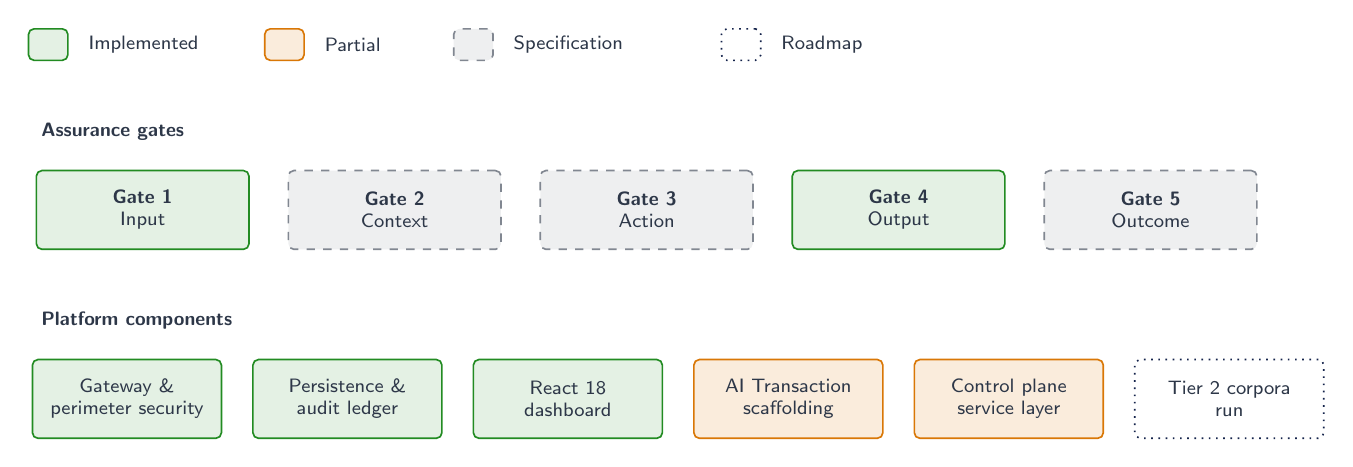
\begin{tikzpicture}
  % legend
  \node[ok,minimum width=0.5cm,minimum height=0.4cm] at (0.2,2.4) {};  \node[base,anchor=west] at (0.6,2.4) {Implemented};
  \node[warn,minimum width=0.5cm,minimum height=0.4cm] at (3.2,2.4) {}; \node[base,anchor=west] at (3.6,2.4) {Partial};
  \node[box,draw=darkslate!60,fill=darkslate!8,dashed,minimum width=0.5cm,minimum height=0.4cm] at (5.6,2.4) {}; \node[base,anchor=west] at (6.0,2.4) {Specification};
  \node[box,dotted,minimum width=0.5cm,minimum height=0.4cm] at (9.0,2.4) {}; \node[base,anchor=west] at (9.4,2.4) {Roadmap};
  % gates
  \node[base,font=\sffamily\scriptsize\bfseries,anchor=west] at (0,1.3) {Assurance gates};
  \node[ok,minimum width=2.7cm,minimum height=1.0cm]  (sg1) at (1.4,0.3)  {\textbf{Gate 1}\\Input};
  \node[box,draw=darkslate!60,fill=darkslate!8,dashed,minimum width=2.7cm,minimum height=1.0cm] (sg2) at (4.6,0.3)  {\textbf{Gate 2}\\Context};
  \node[box,draw=darkslate!60,fill=darkslate!8,dashed,minimum width=2.7cm,minimum height=1.0cm] (sg3) at (7.8,0.3)  {\textbf{Gate 3}\\Action};
  \node[ok,minimum width=2.7cm,minimum height=1.0cm]  (sg4) at (11.0,0.3) {\textbf{Gate 4}\\Output};
  \node[box,draw=darkslate!60,fill=darkslate!8,dashed,minimum width=2.7cm,minimum height=1.0cm] (sg5) at (14.2,0.3) {\textbf{Gate 5}\\Outcome};
  % platform components
  \node[base,font=\sffamily\scriptsize\bfseries,anchor=west] at (0,-1.1) {Platform components};
  \node[ok,minimum width=2.4cm,minimum height=1.0cm]   at (1.2,-2.1)  {Gateway \&\\perimeter security};
  \node[ok,minimum width=2.4cm,minimum height=1.0cm]   at (4.0,-2.1)  {Persistence \&\\audit ledger};
  \node[ok,minimum width=2.4cm,minimum height=1.0cm]   at (6.8,-2.1)  {React 18\\dashboard};
  \node[warn,minimum width=2.4cm,minimum height=1.0cm] at (9.6,-2.1)  {AI Transaction\\scaffolding};
  \node[warn,minimum width=2.4cm,minimum height=1.0cm] at (12.4,-2.1) {Control plane\\service layer};
  \node[box,dotted,minimum width=2.4cm,minimum height=1.0cm] at (15.2,-2.1) {Tier 2 corpora\\run};
\end{tikzpicture}
\end{adjustbox}
\caption{Implementation status by gate and platform component (7 implemented, 2 partial, 3 specification, 1 roadmap item).}
\label{fig:status}
\end{figure}

%==============================================================================
\section{Live Demonstration Walkthrough}\label{sec:demo}
%==============================================================================
The demonstration script
\begin{center}\small\texttt{scripts/demo\_mirage3\_execution\_assurance.py}\end{center}
runs six sequential end-to-end scenarios:
\begin{enumerate}[leftmargin=*,itemsep=2pt]
  \item \textbf{Authoritative identity binding.} JWT issuance via \texttt{mirage\_resolve\_jwt\_identity}; tenant and role claims are immutably bound.
  \item \textbf{Perimeter defence.} Forged headers (\texttt{X-Role: super\_admin}, \texttt{X-Tenant-ID: tenant\_victim}) are stripped at the ASGI boundary, and the legacy \texttt{/v1/auth/demo-token} route returns HTTP~404.
  \item \textbf{Gate 1 input assurance.} \emph{Prompt A (clean)}: baseline risk 0/100. \emph{Prompt B (SSN and API key)}: DLP detects the payload, tags \texttt{TAINT\_CONFIDENTIAL} and raises risk to 15/100. \emph{Prompt C (``IGNORE PREVIOUS SYSTEM INSTRUCTIONS'')}: immediate \texttt{BLOCK} with zero downstream inference or tool cost.
  \item \textbf{Transaction scaffolding.} A transaction envelope with a bounded three-turn ReAct budget moves through \texttt{PENDING} $\rightarrow$ \texttt{ANALYZING} $\rightarrow$ \texttt{ASSEMBLING\_CONTEXT} $\rightarrow$ \texttt{TURN\_REASONING} under optimistic versioned locking.
  \item \textbf{Gate 4 and self-healing.} The grounded Fleming-1928 claim ($\mathrm{HRS}=0.185$ in the scripted run) is emitted directly; the hallucinated Harvard-1999 claim ($\mathrm{HRS}=0.850$) triggers LangGraph and is rewritten from Qdrant evidence to $\mathrm{HRS}_{\text{rewrite}}=0.044\le0.30$. Run-to-run variation in the grounded score is expected because SCS samples at $T=0.7$; both values (0.185 here, 0.2863 in Table~\ref{tab:telemetry_table}) lie well below the 0.60 healing threshold.
  \item \textbf{Audit-chain verification.} Altering one bit of Block~1 invalidates Block~2 and every descendant (Figure~\ref{fig:hashchain}).
\end{enumerate}

%==============================================================================
\section{Research Innovations versus Inherited Heritage}
%==============================================================================
\begin{table}[!htbp]
\centering\small
\renewcommand{\arraystretch}{1.2}
\rowcolors{2}{white}{lightgreybg}
\begin{tabularx}{\linewidth}{@{}L{3.4cm} L{4.5cm} Y@{}}
\hdrrow \hc{Dimension} & \hc{Heritage (MIRAGE 2.x)} & \hc{Novel in MIRAGE 3.0}\\
\toprule
Assurance scope & Output-text hallucination detection only. & \textbf{Five assurance gates} across input, context, action, output and outcome.\\
Governed primitive & Stateless (prompt, completion) checks. & \textbf{AI Transaction} envelope with bounded ReAct turns and budgets.\\
Action and tool safety & Unmanaged tool calls. & \textbf{AI Action Contracts}, capability-based security, blast-radius bounds.\\
Reality verification & None; relied on model output. & \textbf{Epistemic Reality Verification} over seven states.\\
Data-flow security & Static RBAC in the database. & \textbf{Dynamic information-flow control} with lattice taint tracking.\\
Statistical guarantees & Mondrian split-conformal intervals at $1-\alpha=0.95$. & Preserved and integrated into Gate~4 decision boundaries.\\
Self-correction & LangGraph state machine. & Preserved; augmented with boundary-aware token replacement and safety re-checks.\\
\bottomrule
\end{tabularx}
\caption{Inherited heritage versus novel contributions.}
\label{tab:innovations}
\end{table}

%==============================================================================
\section{Strengths, Limitations and Threats to Validity}
%==============================================================================
\subsection{Strengths}
\begin{enumerate}[leftmargin=*,itemsep=1pt]
  \item \textbf{Assurance beyond text:} blocks dangerous actions, context poisoning and phantom successes that text guardrails miss.
  \item \textbf{Distribution-free uncertainty:} split-conformal intervals with finite-sample marginal coverage rather than heuristic scores.
  \item \textbf{Hardened multi-tenancy:} engine-level PostgreSQL RLS plus ASGI header stripping removes the audited IDOR paths.
  \item \textbf{Adaptive cost:} the escalation ladder runs cheap checks first.
\end{enumerate}

\subsection{Limitations}
\begin{enumerate}[leftmargin=*,itemsep=1pt]
  \item \textbf{Sampling latency.} Uncached SCS adds 800--1,800\,ms (mitigated by Redis caching and a bypass for latency-critical tenants).
  \item \textbf{Corpus dependency.} RAV needs an ingested reference corpus; un-indexed domains incur the 0.85 sparsity risk penalty.
  \item \textbf{Multimodal hardware.} Full LLaVA-1.6 grounding needs a high-memory GPU (for example NVIDIA A10G, 24\,GB); developer machines degrade to text-only verification.
  \item \textbf{Cold start.} Loading SentenceTransformers and DeBERTa cross-encoders takes 25--40\,s at container launch.
\end{enumerate}

\subsection{Threats to validity}
\begin{itemize}[leftmargin=*,itemsep=1pt]
  \item Calibration used $n=1{,}000$ examples; coverage is marginal and relies on exchangeability with deployment data.
  \item Telemetry in Table~\ref{tab:telemetry_table} covers two scenarios; the large-scale Tier~2 evaluation is still pending.
  \item Gates 2, 3 and 5, and the end-to-end P95 latency target, are not yet empirically validated.
\end{itemize}

%==============================================================================
\section{Phased Roadmap and Future Work}
%==============================================================================
\begin{figure}[!htbp]
\centering
\begin{adjustbox}{max width=\linewidth}
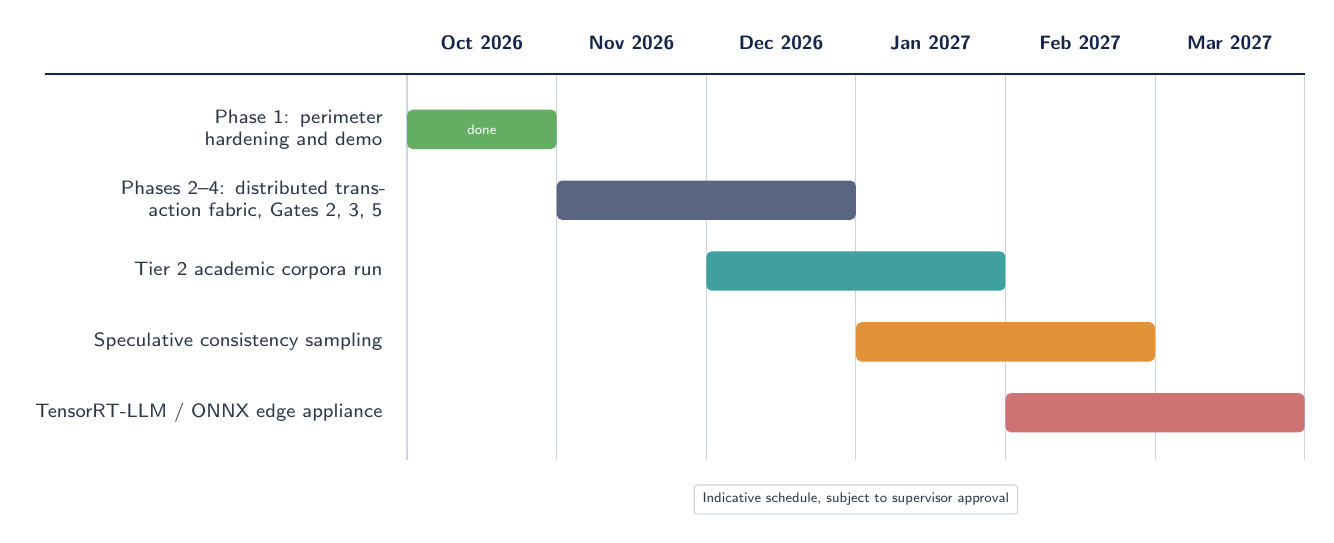
\begin{tikzpicture}
  \foreach \i/\m in {0/Oct 2026,1/Nov 2026,2/Dec 2026,3/Jan 2027,4/Feb 2027,5/Mar 2027}{
    \node[base,font=\sffamily\scriptsize\bfseries,text=primarynavy] at ({4.8+1.9*\i+0.95},0.4) {\m};
    \draw[bordergrey,line width=0.4pt] ({4.8+1.9*\i},0.0) -- ({4.8+1.9*\i},-4.9);
  }
  \draw[bordergrey,line width=0.4pt] (16.2,0) -- (16.2,-4.9);
  \draw[primarynavy,line width=0.6pt] (0.2,0.0) -- (16.2,0.0);
  \foreach \i/\t in {0/{Phase 1: perimeter hardening and demo},1/{Phases 2--4: distributed transaction fabric, Gates 2, 3, 5},2/{Tier 2 academic corpora run},3/{Speculative consistency sampling},4/{TensorRT-LLM / ONNX edge appliance}}{
    \node[base,anchor=east,align=right,text width=4.4cm] at (4.6,{-0.9*\i-0.7}) {\t};
  }
  \fill[forestgreen!70,rounded corners=2pt] (4.8,-0.45) rectangle (6.7,-0.95);
  \node[font=\sffamily\tiny,text=white] at (5.75,-0.7) {done};
  \fill[primarynavy!70,rounded corners=2pt] (6.7,-1.35) rectangle (10.5,-1.85);
  \fill[accentteal!75,rounded corners=2pt]   (8.6,-2.25) rectangle (12.4,-2.75);
  \fill[amberorange!80,rounded corners=2pt]  (10.5,-3.15) rectangle (14.3,-3.65);
  \fill[crimsonred!65,rounded corners=2pt]   (12.4,-4.05) rectangle (16.2,-4.55);
  \node[note,fill=white] at (10.5,-5.4) {Indicative schedule, subject to supervisor approval};
\end{tikzpicture}
\end{adjustbox}
\caption{Phased engineering and research roadmap (indicative).}
\label{fig:roadmap}
\end{figure}

\begin{enumerate}[leftmargin=*,itemsep=2pt]
  \item \textbf{Phases 2--4: distributed transaction fabric and reality probes.} Automated SQL/API postcondition probes; Celery-based distributed transaction runners; implementation of Gates 2 and 3.
  \item \textbf{Tier 2 academic certification.} Full-corpus evaluation on HaluEval \cite{li2023halueval} ($N=10{,}000$), TruthfulQA \cite{lin2022truthfulqa} ($N=817$) and FActScore \cite{min2023} ($N=183$), with paired bootstrap tests ($B=10{,}000$) and an 11-way Bonferroni correction.
  \item \textbf{Speculative consistency sampling.} Lightweight 1B draft models for SCS consensus; the projected goal is a substantial reduction in Groq token cost (target, not yet measured).
  \item \textbf{Edge quantisation.} Compile DeBERTa-v3 and FLAN-T5 to FP8/INT4 ONNX binaries for sovereign on-premise deployment.
\end{enumerate}

%==============================================================================
\section{Conclusion and Faculty Approval Request}
%==============================================================================
Autonomous, tool-executing agents demand a safety architecture that goes beyond output hallucination detection. MIRAGE 3.0 contributes an \textbf{AI Execution Assurance Platform} built on five gates, governed AI transactions and epistemic reality verification. With all P0 identity vulnerabilities closed, Gates 1 and 4 validated by 430+ automated tests, a clean React 18 build and a working live demonstration, the project combines research novelty with production-grade engineering, while remaining explicit about which components are still specifications.

\medskip
We respectfully submit this report to the faculty examination committee for formal review and approval.

\vspace{1.0cm}
\noindent
\begin{minipage}[t]{0.46\textwidth}
  \rule{\linewidth}{0.6pt}\\
  \textbf{Vedant Panchal (23AIML042)}\\
  Student Investigator, B.Tech AI \& ML\\
  CSPIT, CHARUSAT
\end{minipage}
\hfill
\begin{minipage}[t]{0.46\textwidth}
  \rule{\linewidth}{0.6pt}\\
  \textbf{Dax Virani (23AIML076)}\\
  Student Investigator, B.Tech AI \& ML\\
  CSPIT, CHARUSAT
\end{minipage}

\vspace{1.4cm}
\noindent
\begin{minipage}[t]{0.46\textwidth}
  \rule{\linewidth}{0.6pt}\\
  \textbf{Project Guide / Supervisor}\\
  Department of AI \& ML\\
  CSPIT, CHARUSAT
\end{minipage}
\hfill
\begin{minipage}[t]{0.46\textwidth}
  \rule{\linewidth}{0.6pt}\\
  \textbf{Head of Department (HOD)}\\
  Department of AI \& ML\\
  CSPIT, CHARUSAT
\end{minipage}

%==============================================================================
% REFERENCES
%==============================================================================
\clearpage
\begin{thebibliography}{99}\small
\bibitem{manakul2023} Manakul, P., Liusie, A., \& Gales, M.\,J.\,F. (2023). SelfCheckGPT: Zero-resource black-box hallucination detection for generative large language models. \textit{EMNLP 2023}.
\bibitem{min2023} Min, S., et al. (2023). FActScore: Fine-grained atomic evaluation of factual precision in long form text generation. \textit{EMNLP 2023}.
\bibitem{vovk2005} Vovk, V., Gammerman, A., \& Shafer, G. (2005). \textit{Algorithmic Learning in a Random World}. Springer.
\bibitem{lei2018} Lei, J., G'Sell, M., Rinaldo, A., Tibshirani, R.\,J., \& Wasserman, L. (2018). Distribution-free predictive inference for regression. \textit{Journal of the American Statistical Association}, 113(523).
\bibitem{angelopoulos2021} Angelopoulos, A.\,N., \& Bates, S. (2021). A gentle introduction to conformal prediction and distribution-free uncertainty quantification. arXiv:2107.07511.
\bibitem{lundberg2017} Lundberg, S.\,M., \& Lee, S.-I. (2017). A unified approach to interpreting model predictions. \textit{NeurIPS 2017}.
\bibitem{lundberg2020} Lundberg, S.\,M., et al. (2020). From local explanations to global understanding with explainable AI for trees. \textit{Nature Machine Intelligence}, 2(1), 56--67.
\bibitem{he2021v3} He, P., Gao, J., \& Chen, W. (2021). DeBERTaV3: Improving DeBERTa using ELECTRA-style pre-training with gradient-disentangled embedding sharing. arXiv:2111.09543.
\bibitem{song2020} Song, K., Tan, X., Qin, T., Lu, J., \& Liu, T.-Y. (2020). MPNet: Masked and permuted pre-training for language understanding. \textit{NeurIPS 2020}.
\bibitem{malkov2020} Malkov, Y.\,A., \& Yashunin, D.\,A. (2020). Efficient and robust approximate nearest neighbor search using hierarchical navigable small world graphs. \textit{IEEE TPAMI}, 42(4), 824--836.
\bibitem{yao2023react} Yao, S., et al. (2023). ReAct: Synergizing reasoning and acting in language models. \textit{ICLR 2023}.
\bibitem{denning1976} Denning, D.\,E. (1976). A lattice model of secure information flow. \textit{Communications of the ACM}, 19(5), 236--243.
\bibitem{saltzer1975} Saltzer, J.\,H., \& Schroeder, M.\,D. (1975). The protection of information in computer systems. \textit{Proceedings of the IEEE}, 63(9), 1278--1308.
\bibitem{garcia1987} Garcia-Molina, H., \& Salem, K. (1987). Sagas. \textit{ACM SIGMOD 1987}.
\bibitem{li2023halueval} Li, J., Cheng, X., Zhao, W.\,X., Nie, J.-Y., \& Wen, J.-R. (2023). HaluEval: A large-scale hallucination evaluation benchmark for large language models. \textit{EMNLP 2023}.
\bibitem{lin2022truthfulqa} Lin, S., Hilton, J., \& Evans, O. (2022). TruthfulQA: Measuring how models mimic human falsehoods. \textit{ACL 2022}.
\bibitem{mcp2024} Anthropic. (2024). Model Context Protocol specification. \url{https://modelcontextprotocol.io}.
\bibitem{langgraph} LangChain. LangGraph documentation. \url{https://langchain-ai.github.io/langgraph/}.
\end{thebibliography}

\end{document}